\chapter[SegMap-Algorithmus (Schmelzer)]{SegMap-Algorithmus}
\label{sec:SegMap}

Der Segmap-Algorithmus wurde am Autonomous Systems Lab der ETH Zürich ent\-wick\-elt und 2019 im International Journal of Robotics Research veröffentlicht. Die Umgebung wird mit Hilfe eines LiDAR-Sensors in Form einer dreidimensionalen Punkt\-wol\-ke wahrgenommen. Der Algorithmus unterteilt diese in verschiedene Segmente anhand derer sowohl eine Kartierung der Umgebung als auch die Lokalisierung in dieser Karte realisiert wird.

Die Struktur und der Aufbau der Umgebung wird durch Segmente repräsentiert. Dies müssen nicht unbedingt abgeschlossene Objekte sein, sondern können auch nur Teile von Objekten oder Teile größerer Strukturen, wie Fenster oder Türen in Häuserfassaden, sein. Der Vorteil gegenüber der Repräsentation der Umgebung anhand von Objekten ist, dass sich reelle Umgebungen häufig nicht ausschließlich aus tatsächlichen Objekten, die eindeutig unterscheidbar sind, zusammensetzen. Außerdem wird kein perfekter Objektsegmentierungsalgorithmus benötigt. 

Durch die Repräsentation der Umgebung durch Segmente wird die Umwelt im Vergleich zur gesamten Punktwolke deutlich kompakter aber dennoch unterscheidbar darstellt. Außerdem wird zur weiteren Verarbeitung der Segmente deutlich weniger Rechenkapazität benötigt im Vergleich zur dreidimensionalen Punktwolke. Für jedes Segment wird durch einen Deskriptor in Form eines CNNs ein kompakter Merkmalsvektor erstellt, der dieses möglichst eindeutig beschreibt. Dadurch wird eine zusätzliche Kompression der Segmente erreicht und eine Szene kann effektiv zusammengefasst werden mit ein paar kompakten Merkmalsdeskriptoren. Zusätzlich ist es möglich durch Dekodierung des Merkmalsvektors eine dreidimensionale Karte, die aus Segmenten aufgebaut ist, zu rekonstruieren. 

Durch die enorme Kompression der Punktwolke auf ein paar Merkmalsvektoren, verringert sich der Speicherbedarf sowie die benötigte Rechenkapazität für die Weiterverarbeitung deutlich gegenüber der gesamten Punktwolke. Außerdem müssen bei\-spiels\-wei\-se bei Multi-Robot-Anwendungen weniger Daten übertragen werden, wodurch dies beschleunigt und weniger Bandbreite benötigt wird. Durch die Möglichkeit der Dekodierung von Kartendaten aus den Merkmalsvektoren, kann effizient visuelles Feedback an Enduser geliefert werden, wie z.B. an den Bediener eines Roboters bei Such- und Rettungsmanövern. Außerdem wird das System dadurch echtzeitfähig. 

Die Lokalisierung und damit auch das Erkennen von Loop Closures wird durch das Finden von Paaren der selben Segmente in der lokalen Punktwolke und in der Karte realisiert. Die Merkmalsvektoren der Segmente werden miteinander verglichen und so potentielle Paare gefunden. Eine Loop Closure wird erkannt, wenn eine festgelegte Anzahl an Paaren in einem Bereich der Karte gefunden wurde und die geometrischen Beziehungen zwischen diesen Segmenten in der lokalen Punktwolke mit denen in der Karte übereinstimmen. Nach einer erkannten Loop Closure wird die Trajektorie neu geschätzt und die Karte angepasst. Dadurch wird unvermeidbarer Drift in der Odometrie korrigiert und somit eine genauere Kartierung ermöglicht. 

Mit einem weiteren KNN können zusätzlich semantische Informationen jedes Segments aus den Merkmalsvektoren extrahiert werden durch eine Klassifikation im Merkmalsraum. Diese Informationen verbessern beispielsweise die   Robustheit gegenüber Änderungen in der Umgebung. Eine bereits realisierte Anwendung hierzu ist bei outdoor-Szenarien keine Autos zur Lokalisierung zu verwenden. 

Der Segmap-Algorithmus ist parametrisiert für urbane outdoor-Anwendungen mit einem LiDAR-Sensor. Das Training des Segmentdeskriptors sowie die Evaluierung des SegMap-Algorithmus wurde anhand des KITTI Odometrie Datensatzes durchgeführt. Hierbei wurden für das Training und die Evaluierung verschiedene Sequenzen des Datensatzes gewählt, um eine unabhängige Evaluierung zu gewährleisten. Die Ergebnisse zeigen, dass der SegMap-Ansatz gute Ergebnisse erzielt und eine zuverlässige Lokalisierung möglich ist. Außerdem ist das Erkennen von Loop Closures sowie das anschließende Anpassen der Trajektorie und der Karte in Echtzeit möglich. 

Der Algorithmus ist modular aufgebaut, um leichter Teile des Codes ersetzen oder ändern zu können. Abbildung \ref{fig:segmap} zeigt die Architektur des Verfahrens und die Schnittstelle zum einem Laser-SLAM Framework. 

\begin{figure}
    \centering
    \includegraphics[width=\linewidth]{Bilder/segmap_aufbau.png}
    \caption{Modularer Aufbau des Segmap-Algorithmus \cite{Dube2018}}
    \label{fig:segmap}
\end{figure}

Im weiteren Verlauf des Kapitels werden die einzelnen Elemente, aus denen der Algorithmus sich zusammensetzt, detailierter beschrieben. 

%\section[Aufbau (Schmelzer)]{Aufbau}
%\label{sec:SegMap Aufbau}
%
%Der SegMap-Algorithmus ist modular aufgebaut, um leichter Teile des Codes ersetzen oder ändern zu können. Abbildung \ref{fig:segmap} zeigt die Architektur des Verfahrens und die Schnittstelle zum einem Laser-SLAM Framework. 
%
%\begin{figure}
%    \centering
%    \includegraphics[width=\linewidth]{Bilder/segmap_aufbau.png}
%    \caption{Modularer Aufbau des Segmap-Algorithmus \cite{Dube2018}}
%    \label{fig:segmap}
%\end{figure}

\section[Filterung und Registrierung (Schmelzer)]{Filterung und Registrierung}
\label{sec:Filterung}

Zu Beginn werden im Laser-SLAM Framework die eingehenden Punktwolken über ICP gegeneinander registriert \cite{Dube2018}. Dadurch wird eine Transformation zwischen den aufeinander folgenden Roboterposen bestimmt. Diese wird zusätzlich zu Hardware-basierten  Odometrieinformationen der Roboterplattform zur Ermittlung einer Posenschätzung verwendet.  

Anschließend wird aus der eingehenden dreidimensionalen Punktwolke eine lokale Punktwolke erzeugt. Hierfür wird ein Zylinder mit Radius $ R $ um die aktuelle Roboter Position definiert und alle Punkte, die außerhalb dieses Zylinders liegen, werden verworfen.  In z-Richtung wird die Höhe des Zylinders durch die angegebene minimale und maximale Höhe eines Punktes begrenzt. Außerdem werden durch die bekannte Höhe des Sensors über dem Boden alle Punkte unterhalb dieser Höhe entfernt. Diese bilden den Boden. Dieser muss aus der Punktwolke entfernt werden, damit nicht die gesamte Umgebung zu einem riesigen Segment wird. 

\section[Dynamisches Voxelgitter (Schmelzer)]{Dynamisches Voxelgitter}
\label{sec:DVG}

Der einkommende kontinuierliche Strom aus dreidimensionalen Punktwolken wird zuerst in einem regelmäßigen dreidimensionalen Voxelgitter zusammengefasst \cite{Dube2018}. Abhängig von der Kantenlänge des Voxelgitters, kann jedes Voxel mehrere Punkte beinhalten. Aus allen Punkten in einem Voxel werden für alle Voxel die jeweiligen Schwerpunkte berechnet. Anstatt dies bei jeder neuen Messung zu wiederholen, werden immer nur die Werte der Voxel neu berechnet, zu denen neue Punkte hinzukommen. Dadurch wird Rechenkapazität gespart und der Prozess wesentlich beschleunigt gegenüber einer ständigen Verarbeitung der gesamten Punktwolke. Durch das dynamische Hinzufügen und Entfernen von Punkten aus dem Voxelgitter, handelt es sich um ein dynamisches Voxelgitter. 

Ein Voxel gilt als belegt, wenn es eine Mindestanzahl an Punkten enthält. Dadurch wird Rauschen reduziert.  Für die weitere Verarbeitung der Punktwolke wird diese auf die belegten Voxel reduziert. Da jedes Voxel mehrere Punkte enthalten kann, wird die Punktwolke somit von deutlich weniger Punkten repräsentiert. Dadurch wird zusätzlich Speicherplatz und Rechenkapazität gespart. Jedes Voxel fasst die Lage aller enthaltenen Punkte anhand seines Schwerpunkts zusammen. Alle belegten Voxel werden in einem Vektor in aufsteigender Voxel-Index-Folge gespeichert. Jeder Voxel trägt neben seinem Index zusätzlich auch die Information über die Lage seines Mittelpunkts sowie die Anzahl der Punkte, die er umfasst. 

Die Auflösung $ r $ des regelmäßigen Voxelgitters wird über die Kantenlänge der Voxel definiert, die in allen drei Dimensionen identisch ist. Das Gitter hat eine Größe von $ l \times w \times h $ Voxeln. Jedes Voxel hat einen eindeutigen Index im Bereich von $ [0,l \cdot w \cdot h -1] $. Über die euklidische Transformation $ T_{mg} $ vom Koordinatensystem des Voxelgitters in das der Karte wird eine Beziehung zwischen beiden Koordinatensystemen hergestellt. Initialisiert ist diese so, dass der Roboter im Mittelpunkt des Voxelgitters startet.  

Für jeden neuen Punkt $ q $ wird der Index des Voxels berechnet, dem er zugeordnet wird.  Hierfür werden zuerst die Koordinaten $ t $ des Punktes im Koordinatensystem des Voxelgitters berechnet: 

\begin{align}
	t = T_{mg}^{-1} \cdot q \cdot r^{-1}
\end{align}

Aus Gründen der Recheneffizienz muss die Größe des Voxelgitters in allen drei Dimensionen eine Zweierpotenz sein. Daraus ergibt sich: $ l = 2^{l_{bits}}, w = 2^{w_{bits}} $ und $ h = 2^{h_{bits}} $. Die Indizes werden als $ b $-Bit unsigned Integer gespeichert mit $ b \geq (l_{bits} + w_{bits} + h_{bits}) $. Mit diesen Bedingungen wird der Index $ I(q) $ eines neuen Punktes $ q $ berechnet mit: 

\begin{align}
	I(q) = \lfloor t.x \rfloor + \lfloor t.y \rfloor \ll l_{bits} + \lfloor t.z \rfloor \ll (l_{bits} + w_{bits})
\end{align}

wobei $ \ll $ der Operator für eine bitweise Verschiebung nach links ist. 

Nachdem für alle neuen Punkte der jeweilige Voxel-Index berechnet wurde, werden diese in aufsteigender Voxel-Index-Folge sortiert und in einem Vektor gespeichert. Da Sortieren eine asymptotische Komplexität von $ O(n log (n)) $ hat, ist es eine wesentliche Verbesserung nur die neuen Punkte zu beachten anstatt die gesamte Punktwolke erneut den jeweiligen Voxeln zuzuordnen.  Anschließend werden die Punkte in linearer Zeit dem jeweiligen Voxel hinzugefügt, dem sie anhand des Index zugeordnet wurden. Hierfür wird für jeden Voxel, dem $ m $ neue Punkte $ q_i $ hinzugefügt werden, ein neuer Schwerpunkt berechnet und anschließend die Anzahl $ n $ der in ihm enthaltenen Punkte aktualisiert:  

\begin{align}
	p \leftarrow \left( n \cdot p + \sum_{i=1}^{m} q_i \right) \cdot \frac{1}{n + m}, \qquad n \leftarrow n + m
\end{align}


Voxel, die erst in der aktuellen Messung genügend Punkte umfassen, um als belegt zu gelten, werden zusätzlich in einer Menge $ U $ gesammelt. Dies ermöglicht es, in den weiteren Verarbeitungsschritten lediglich mit einer relativ kleinen Untermenge der Voxel zu arbeiten und somit redundante Berechnungen zu sparen.

Sobald der Roboter sich weiterbewegt, werden die Voxel entfernt, die durch die Bewegung außerhalb des Radius der lokalen Karte fallen, während auf der anderen Seite neue Voxel hinzukommen.

Da es sich um ein SLAM-Verfahren handelt, wird im Falle einer Loop Closure die Trajektorie des Roboters neu berechnet und eine neue Pose geschätzt. Auch die lokale Karte muss an diese neue Posenschätzung angepasst werden. Dafür wird die euklidische Transformation der bisherigen Pose auf die neu geschätzte Pose auch auf die Voxel-Schwerpunkte angewandt. Daraus ergibt sich, dass auch die Transformation $ T_{mg} $ vom Koordinatensystem des Voxelgitters auf das der Karte angepasst werden muss, damit die neuen Punkte der nächsten Messung auch weiterhin den richtigen Voxeln zugeordnet werden. Die Transformation wird aktualisiert durch $ T_{mg} \leftarrow TT_{mg} $.  

\section[Inkrementelle Normal- und Krümmungsschätzung (Schmelzer)]{Inkrementelle Normal- und Krümmungsschätzung}

Für jeden Voxel-Schwerpunkt wird sowohl die Normale als auch die Krümmung der benachbarten Region berechnet, da diese für die Segmentierung benötigt werden \cite{Dube2018}. Hierbei werden nur die Voxel verwendet, die bei der letzten Messung aktiviert wurden. 

Die Nachbarschaft $ \mathcal{N}(p_i) $ des Punktes $ p_i $ wird mittels einer Nearest Neighbors (NN) Suche mit einem festen Radius ermittelt und die Punkte in ein $ n_i $-Tupel $ \{v_j\}_{j=1}^{n_i} := \mathcal{N}(p_i) $ angeordnet. Im Allgemeinen wird die Normale eines Punktes $ p_i $ einer dreidimensionalen Punktwolke anhand der Kovarianzmatrix $ M_i $ seiner Nachbarschaft berechnet:

\begin{align}
	\label{kovarianmatrix}
	M_i := \overline{(v_j-\overline{v})(v_j-\overline{v})^T}
\end{align}

Hierbei stellt $ \overline{\cdot} $ die Berechnung des Mittelwerts dar. Daraus ergibt sich $ \overline{v_j} := \frac{1}{\vert v \vert} \sum_{j=1}^{\vert v \vert} v_j $, wobei der Index auch weggelassen werden kann. Die Schätzung der Normalen entspricht dem normierten Eigenvektor von $ M_i $   bezüglich des kleinsten Eigenwertes. Die Krümmung $ \sigma $ wird ebenfalls anhand der Eigenwerte $ \lambda_0 < \lambda_1 < \lambda_2 $ von $ M_i $ berechnet mit $ \sigma = \lambda_0(\lambda_0+\lambda_1+\lambda_2)^{-1} $. 

Um die Schätzungen der Normale und der Krümmung inkrementell berechnen zu können, muss auch die Kovarianzmatrix $ M_i $ inkrementell berechnet werden durch Anpassung der Gleichung \ref{kovarianmatrix}:

\begin{align}
	M_i = \overline{v_jv_j^T}-\overline{v}\overline{v^T} = \frac{1}{n_i}\cdot A_i-\frac{1}{n_i^2}\cdot b_ib_i^T
\end{align} 
 
Hierbei ist $ A_i $ der Akkumulator von $ \overline{v_jv_j^T} $ und $ b_i $ der Akkumulator von $ \overline{v} $. Dadurch kann die Kovarianmatrix inkrementell berechnet werden, ohne die Nachbarschaft  $ \mathcal{N}(p_i) $ jedes Punktes tracken zu müssen. 

Die Akkumulatoren jedes Punktes werden inkrementell mit Hilfe eines Scattering and Gathering Verfahrens der jeweiligen Beiträge berechnet. Für jeden neuen Punkt werden $ A_i, b_i $ und $ n_i $ mit 0 initialisiert und anschließend für jeden Punkt $ p_j \in \mathcal{N}(p_i) $, die jeweiligen Beiträge gestreut: 

\begin{align}
	A_j \leftarrow  A_j + p_ip_i^T, \qquad b_j \leftarrow b_j + p_i, \qquad n_j \leftarrow n_j + 1
\end{align}

Anschließend werden ausschließlich die Beiträge alter Punkte wieder gesammelt: 

\begin{align}
	A_i \leftarrow A_i + p_jp_j^T, \qquad b_i \leftarrow b_i + p_j, \qquad n_i \leftarrow n_i + 1
\end{align}

Die  Kovarianzmatrizen, Normalen und Krümmungen werden erneut berechnet für die Punkte, deren Akkumulatoren sich geändert haben.

Im Fall einer Loop Closure wird eine euklidische Transformation auf alle Voxel angewendet. Diese Transformation muss ebenfalls auf die Akkumulatoren angewendet werden, um Fehler zu vermeiden durch das Akkumulieren von Punkten, die zu verschiedenen Koordinatensystemen gehören. Die Transformation, die auf alle Punkte der lokalen Punktwolke angewendet wird, wird durch eine Rotation $ R $ mit anschließender Translation $ t $ ausgedrückt mit $ p_i \leftarrow Rp_i  t $. Daraus ergibt sich das transformierte Tupel der Nachbarschaft des Punktes $ p_i $ $ \widetilde{v} := (Rv_j + t)_{j=1}^{n_i} $. Die transformierte Kovarianzmatrix kann unter Verwendung folgender Gleichungen berechnet werden: 

\begin{align}
	\overline{\widetilde{v}_j \widetilde{v}_j^T} = R\overline{v_jv_j^T}R^T  R\overline{v}t^T  + t\overline{v}^TR^T + tt^T
\end{align}

\begin{align}
		\overline{\widetilde{v}} = \overline{Rv_j+t} = R\overline{v}+t
\end{align}

Die Akkumulatoren werden  aktualisiert mit: 

\begin{align}
	A_i \leftarrow RA-iR^T+Rb_it^T+tb_i^TR^T+n_itt^T,  \qquad b_i \leftarrow Rb_i+n_it
\end{align}
 
Die Normalen werden aktualisiert mit: $ N_i \leftarrow RN_i $, während die Krümmungen von den Transformationen nicht beeinflusst werden. 
 
\section[Inkrementelle Segmentierung durch Region Growing (Schmelzer)]{Inkrementelle Segmentierung durch Region Growing}
\label{sec:Segmentierung}

Aus der Punktwolke, die aus den Schwerpunkten der Voxel besteht, werden durch das bilden von Clustern Segmente extrahiert \cite{Dube2018}. Hierfür wird eine Clustering-Methode verwendet, die in der Lage ist wiederholt die selben Segmente aus einer Punktwolke zu bilden. Verwendet wird ein inkrementeller Region Growing Algorithmus, der nur auf die Voxel angewendet wird, die in der letzten Messung belegt wurden. Abbildung \ref{fig:bsp_segmentierung} zeigt drei Beispiele von Segmenten, die inkrementell über mehrere Beobachtungsschritte $ k $ wachsen.

\begin{figure}
    \centering
    \includegraphics[width=\linewidth]{Bilder/segmente_ink_grow.png}
    \caption{Beispiele inkrementell gewachsener Segmente über mehrere aufeinander folgende Beobachtungen \cite{Dube2018}}
    \label{fig:bsp_segmentierung}
\end{figure}

Segmente beginnen von einem Startpunkt aus zu wachsen, indem unter Beachtung bestimmter Regeln Cluster mit den benachbarten Punkten gebildet werden. Sobald alle Punkte Clustern, die jeweils eine individuelle Cluster-ID haben, zugewiesen wurden, werden Cluster, die eine bestimmte Mindestanzahl an Punkten überschreiten, als Segment mit einer individuellen Segment-ID in die Karte geschrieben. Die Startpunkte, von denen Segmente beginnen zu wachsen, werden Samen (Seeds) genannt und in einer Liste gespeichert. Anschließend wird auf jeden dieser Punkte der Region Growing Algorithmus angewendet, dessen Pseudocode in Algorithmus \ref{Segmentierung} gezeigt ist. 
  
\floatname{algorithm}{Algorithmus}
\begin{algorithm}
	\caption{Inkrementelles Region Growing mit gegebenem Anfangssamen, einer Punktwolke P und einer neuen Cluser-ID $ \gamma $ \cite{Dube2018}.}
	\label{Segmentierung}
	\begin{algorithmic}[1]
		\Function{GROWFROMSEED}{$s,P,\gamma$}
			\State $ \Gamma \leftarrow \{s\}, S \leftarrow \{s\} $ // Initialisiere Cluster und Menge der Samen
			\While{$ Samen \neq \emptyset $} 
				\State $ s \leftarrow POPFRONT(S) $
				\ForEach{$ n $ : NN($ s,P $)}
					\If{CANGROWTO($ s,n $)}
						\If{HASCLUSTERID($ n $)}
							\State LINKCLUSTERS($ s,n,\gamma $)
						\Else
							\State SETCLUSTERID($ n,\gamma $)
							\State $ \Gamma \leftarrow \Gamma \cup \{n\} $
							\If{CANBESEED($ n $)}
								\State $ S \leftarrow S \cup \{n\} $
							\EndIf
						\EndIf
					\EndIf
				\EndFor
			\EndWhile 
			\State \Return{$ \Gamma $}
		\EndFunction
	\end{algorithmic}
\end{algorithm}

Das Clustern beginnt mit einem Punkt $ s $ der Liste der Samen. Die Funktion NN ermittelt anhand einer Suche mit festem Radius die benachbarten Punkte des Samens. Hierfür wird der selbe $k$-d-Baum verwendet, wie bereits bei der Normalen- und Krümmungsschätzung. In einer Schleife wird für jeden Punkt seiner Nachbarschaft anhand der Verwendeten Regel für das Growing geprüft, ob das Wachsen vom Samen zu diesem Punkt erlaubt ist. Wenn das zusammenwachsen erlaubt ist und dem Punkt bereits eine Cluster-ID $ \gamma $ zugeordnet ist, werden die Cluster beider Punkte miteinander verbunden. Andernfalls wird der Punkt dem Cluster des Samens hinzugefügt und dieselbe Cluster-ID gegeben. Wenn der Punkt die Voraussetzungen erfüllt ein Samen zu sein, wird dieser in eine Liste geschrieben, deren Punkte nacheinander in einer Schleife die gleichen Cluster-Schritte durchlaufen wie der ursprüngliche Samen $ s$. Dadurch wächst das Cluster ausgehend vom Startpunkt durch Streuung der Samen immer weiter, bis keine weiteren Punkte mehr in der Nachbarschaft liegen, die als Samen verwendet werden können. Die Ausgabe ist ein Cluster $ \Gamma $, dem alle Punkte zugewiesen sind, die durch den Region Growing Algorithmus vom Startpunkt $ s $ aus erreicht wurden. 

Es werden zwei verschiedene Region Growing Ansätze verwendet, zwischen denen gewählt werden kann. Diese unterscheiden sich in den  Regeln, auf Basis derer die Cluster gebildet werden. 

Der erste Ansatz clustert Punkte zusammen, die eine ebene Fläche bilden. Es werden nur Punkte als Samen verwendet, deren Krümmung unterhalb eines bestimmten Grenzwerts liegt. Die Samen werden nach aufsteigender Krümmung sortiert. Dadurch beginnen die Segmente von den flachsten Punkten aus zu wachsen, wodurch die Anzahl der zu bildenden Cluster reduziert wird. Außerdem können nur Punkte zusammenwachsen, deren Normalen annähernd parallel sind. Da allerdings die Orientierung der Normalen nicht bekannt ist, wird diese durch die Vorgabe approximiert, dass das Kreuzprodukt beider Normalen unter einem vorgegeben Grenzwert liegen muss. 

Der zweite Ansatz für das Growing basiert auf euklidischen Distanzen. Hierbei werden alle Punkte, die keinem Cluster zugewiesen sind, unabhängig von ihrer jeweiligen Krümmung als Samen verwendet. Es können alle Punkte zusammenwachsen, deren euklidischer Abstand unter einem vorgegeben Grenzwert liegt.

Abbildung \ref{fig:cluster_merging} verdeutlicht den Region Growing Algorithmus auf Basis euklidischer Distanzen anhand eines zweidimensionalen Beispiels. Der Grenzwert für den eu\-kli\-disch\-en Abstand zwischen zwei Punkten bildet einen Kreis um den Samen. Alle Punkte, die innerhalb dieses Kreises liegen, bilden ein Cluster. Im ersten Teil der Abbildung (a) wird ausgehend vom Samen ein Punkt erreicht, der noch keinem Cluster zugewiesen ist. Dieser wird daher zum Cluster des Samens hinzugefügt. In (b) und (c) werden bereits existierende Cluster erreicht und mit dem wachsenden Cluster zusammengeführt. Alle Punkte erhalten die selbe Cluster-ID. Falls zusammenwachsende Cluster bereits beide eine gültige Segment-ID haben, erhält das resultierende Segment die kleinste beider Segment-IDs, da diese die ältere ist. Anschließend werden auch die Segment-IDs in der Karte entsprechend aktualisiert. Somit wird das bilden von Segment-Duplikaten in der Karte verhindert und dadurch eine robustere Lokalisierung ermöglicht. 

\begin{figure}
    \centering
    \includegraphics[width=\linewidth]{Bilder/region_growing.png}
    \caption{Zweidimensionale Darstellung des Region Growing und Merging mit euklidischen Distanzen \cite{Dube2018}}
    \label{fig:cluster_merging}
\end{figure}

Im Gegensatz zu den Cluster-IDs sind die Segment-IDs beständig und werden nicht neu vergeben, wenn Segmente miteinander verschmelzen. Stattdessen werden die IDs, die in diesem Schritt wegfallen verwendet, um die Entwicklung der Segmente über die verschiedenen Messungen zu verfolgen und als Menge vergangener Beobachtungen $ S_i = \{s_1,s_2,...,s_n\} $ gespeichert. Hierbei ist jede Beobachtung $ s_j \in S_i $ des Segments eine dreidimensionale Darstellung in Form einer Punktwolke, die zeigt, wie das Segment zum Zeitpunkt der Messung ausgesehen hat. Hierbei stellt $ s_n $ die aktuellste Beobachtung des Segments dar. Mit jeder Messung kommen weitere Punkte zu den Segmenten hinzu. Ein Segment ist abgeschlossen, wenn keine weiteren Punkte mehr hinzukommen, da der Roboter weiter gefahren ist.  Die verschiedenen Entwicklungsstadien der Segmente werden für das Training des Deskriptors verwendet, um robuster gegen Blickwinkeländerungen zu werden.

Abbildung \ref{fig:evolution_segmente} verdeutlicht anhand eines Beispiels, wie Segmente sich über mehrere Messungen entwickeln, während der Roboter fährt. Der schwarze Kreis um den Roboter symbolisiert die Grenze der lokalen Karte. In diesem Beispiel muss ein Cluster mindestens aus drei Punkten bestehen, um ein Segment zu bilden. Bei der ersten Messung (a) erkennt der Roboter ein Segment und ein Cluster. Das Segment ist blau gefärbt und das Cluster orange. In (b) ist der Roboter weiter gefahren, wodurch neue Punkte zu den Beobachtungen dazu kommen. Seine lokale Karte enthält nun ein weiteres Cluster, das grün gefärbt ist. Das orange Cluster ist zu einem Segment geworden und das blaue Segment ist gewachsen mit gleichbleibender Segment-ID. Im letzten Schritt (c) ist der Roboter noch weiter gefahren. Durch den anderen Blickwinkel wurden neue Punkte erkannt, die das blaue und orange Segment verbunden haben. Beide Segmente sind zusammengewachsen und haben die ID des älteren Segments, in dem Fall die des blauen, übernommen. Außerdem ist das grüne Cluster zu einem Segment herangewachsen.  

\begin{figure}
    \centering
    \includegraphics[width=\linewidth]{Bilder/segment_growing.png}
    \caption{Beispielhafte Darstellung der Entwicklung und des trackings von Segmenten während der Roboter sich bewegt \cite{Dube2018}}
    \label{fig:evolution_segmente}
\end{figure}

\section[Deskriptor (Kopp)]{Deskriptor}
\label{sec:Deskriptor}

Mit Hilfe eines CNNs werden die Segmente  auf einen kompakten Deskriptor in Form eines Merkmalsvektors komprimiert, der diese möglichst eindeutig beschreibt \cite{Dube2019}. Abbildung \ref{fig:deskriptor} zeigt die Architektur des CNNs. Die Eingabe des CNNs ist das zu beschreibende Segment, das in ein dreidimensionales Voxelgitter mit einer festen Größe von $ 32 \times 32 \times 16 $ Voxel eingefügt wird. Die Dimension der Eingabe wurde empirisch ermittelt, um einen guten Kompromiss zwischen Deskriptionsfähigkeit und der Größe des Netzwerkes zu schaffen. Der Descriptor Extractor besteht aus drei dreiminesionalen Convolutional Layern (Conv) zwischen denen insgesamt zwei MaxPooling Layer (MaxPool) angeordnet sind. Abgeschlossen wird das CNN von zwei Fully Connected Layern (FC), die durch ein Batch Normalization Layer (BN) verbunden sind und mit einem Dropout von 50\% trainiert werden. Bei allen Schichten wird die ReLU-Aktivierungsfunktion verwendet. Die Aktivierungen des letzten Fully Connected Layers bilden den Segment-Deskriptor mit einer Dimension von $ 64 \times 1 $. Mit dem angehangenen Decoder Netz zur Rekonstruktion der Segmente aus deren jeweiligen Deskriptoren bildet der Deskriptor Extractor einen Autoencoder. Eine Rastersuche über verschiedene Parameter und Netzkonfigurationen hat gezeigt, dass diese Netzarchitektur die besten Ergebnisse liefert. 

\begin{figure}
    \centering
    \includegraphics[width=\linewidth]{Bilder/deskriptor.png}
    \caption{Darstellung der Struktur des Deskriptor-Autoencoders \cite{Dube2019}}
    \label{fig:deskriptor}
\end{figure}

Auf Abbildung \ref{fig:deskriptor} geben die Parameter der Convolutional und Deconvolutional Layer die Anzahl der Filter sowie deren Größen an, die der MaxPooling Layer die Größe der Pooling Operation und die der Fully Connected Layer die Anzahl der Neuronen.

Bevor die Segmente dem Descriptor Extractor zugeführt werden, werden sie mit Hilfe einer zweidimensionalen PCA einheitlich ausgerichtet, um robuster gegen Blickwinkeländerungen zu werden. Die PCA wird auf alle Punkte des Segments angewendet. Unter der Annahme, dass die z-Achse des Koordinatensystems des Segments mit der Gravitation ausgerichtet ist, wird das Segment so rotiert, dass die x-Achse seines Koordinatensystems aus der Perspektive des Roboters in die selbe Richtung wie der Eigenvektor des größten Eigenwertes zeigt. Die Mehrdeutigkeit in der Ausrichtung wird gelöst, indem das Segment so rotiert wird, dass der untere Teil des Segments entlang seiner y-Achse die höhere Anzahl an Punkten enthält. 

Segmente werden so in das Voxelgitter geschrieben, dass der Schwerpunkt des ausgerichteten Segments mit dem Mittelpunkt des Voxelgitters übereinstimmt. Die Voxel haben eine minimale Kantenlänge von 0,1m, die allerdings individuell erhöht werden kann, damit auch Segmente, die größer als das Voxelgitter sind, hineinpassen. Die Skalierung der Segmente über eine minimale Kantenlänge ist im Vergleich zur Skalierung der Größe des Segmentes anhand eines Seitenverhältnisses robuster gegen Aliasing. Außerdem werden bessere Ergebnisse bei der Rekonstruktion der Segmente erreicht. Der Einfluss auf die Wiedererkennung der Segmente bei der Lokalisierung wird minimiert indem die Originalskalierung des Segmentes als zusätzlicher Parameter dem ersten Fully Connected Layer des Descriptor Extractors zugeführt wird. 

Der Autoencoder muss so trainiert werden, dass sowohl die Wiedererkennungrate der Segmente bei der Lokalisierung möglichst hoch ist, als auch dass die Rekonstruktionen so genau wie möglich den Originalsegmenten entsprechen. Wie auf Abbildung \ref{fig:deskriptor} gezeigt, wird der Descriptor Extractor um eine Klassifikationsschicht mit der Softmax-Aktivierungsfunktion erweitert. Diese wird lediglich zum Trainieren der Wiedererkennung von Segmenten verwendet und anschließend verworfen. Angewendet wird eine Lernmethode, die ähnlich ist zu dem \textit{N-ways classification problem} \cite{Parkhi2015}. Die Trainingsdaten werden in $ N $ Klassen eingeteilt. Eine Klasse enthält alle Beobachtungen eines Segmentes oder mehrerer Segmente, die zum gleichen Objekt oder Teil der Umgebung gehören. Auch diese Klassen werden lediglich für das Training gebraucht und stehen in keinem Zusammenhang mit der Extraktion der semantischen Informationen. Während dem Training weist das Netz bei jedem Segment des Trainingsdatensatzes jeder der $ N $ Klassen einen Score zu, der angibt mit welcher Wahrscheinlichkeit das Segment zur jeweiligen Klasse gehört. Anschließend werden diese Scores  mit dem tatsächlichen Klassen-Label des Trainingsdatensatzes über den \textit{softmax cross entropy loss} verglichen und der Klassifikationsverlust  $ L_c $ berechnet:

\begin{align}
	L_c = -\sum_{i=1}^{N} y_i log\frac{e^{l_i}}{\sum_{k=1}^{N} e^{l_k}}
\end{align}

In der Formel stellt $ y $ den One-Hot kodierten Vektor der tatsächlichen Klassenlabel und $ l $ die Ausgabe der Klassifikationsschicht dar. One-Hot kodiert bedeutet, dass der Vektor nur an der Stelle des tatsächlichen Klassen-Labels eine Eins enthält und ansonsten mit Nullen gefüllt ist. Durch eine hohe Anzahl an Klassen und die geringe Dimension des Merkmalsvektors wird der Descriptor Extractor gezwungen besser zu generalisieren und so Overfitting zu bestimmten Segment Samples vermieden.

Wie bereits erwähnt, können Segmente mithilfe des angehangenen Dekodernetzes aus dem Deskriptor rekonstruiert werden. Wie auf Abbildung \ref{fig:deskriptor} dargestellt, besteht das Dekodernetz aus einem Fully Connected Layer, das ReLU als Aktivierungsfunktion verwendet, und drei Deconvolutional Layern (Deconv). Auch hier wird bei allen Schichten die ReLU-Aktivierungsfunktion verwendet. Ausnahme ist die letzte Schicht, bei der die Sigmoid-Aktivierungsfunktion gewählt wurde. Zwischen dem Enkoder und Dekoder Netz werden keine Gewichte geteilt. Beim Training wird eine spezielle Form des \textit{binary cross entropy loss} verwendet, um den Verlust $ L_r $ der Rekonstruktionen zu berechnen \cite{Brock2016}: 

\begin{align}
	L_r = -\sum_{x,y,z}(\gamma t_{xyz}log(o_{xyz}) + (1 - \gamma)(1 - t_{xyz})log(1 - o_{xyz}))
\end{align}
 
In der Formel ist $ t $ das Target-Segment und $ o $ die Ausgabe des Netzes. Der Hyperparameter $ \gamma $ gewichtet die  relative Wichtigkeit von fasch Negativen und falsch Positiven Ausgaben, da nur eine geringe Anzahl Voxel der Voxelgrid pro Segment belegt ist. Bei den Verwendeten Trainingsdaten waren durchschnittlich nur 3\% der Voxel belegt und mit $ \gamma = 0.9 $ wurden gute Ergebnisse erzielt. 

Beide Fähigkeiten werden simultan trainiert. Hierfür werden die Verluste beider Loss-Funktionen summiert, wobei der Parameter $ \alpha $ die relative Wichtigkeit beider Verluste gewichtet: 

\begin{align}
	L = L_c + \alpha L_r
\end{align}

Es wurde empirisch festgestellt, dass mit $ \alpha = 200 $ die Leistung des simultan trainierten Netzes im Vergleich zu einem separaten Training mit jeweils einer der beiden Loss-Funktionen nicht signifikant beeinflusst wird. 

Die Initialisierung der Gewichte erfolgt mittels Xaviers Initalisierungsmehtode \linebreak \cite{Glorot2010}.
Trainiert wird mit Hilfe des Adaptive Moment Estimation (ADAM) optimizer mit einer Lernrate von $ 10^{-4} $ \cite{Kingma2014}.  Hierbei werden im Gegensatz zur stochastischen Gradientenabstieg separate Lernraten für jeden Parameter des Netzes geführt, wodurch das simultane Training zwei verschiedener Fähigkeiten erleichtert wird. Mit Hilfe von einem Dropout von 50\% und Batch Normalization wird Regularisierung erreicht. 

SegMap bietet zusätzlich die Möglichkeit einen Deskriptor auf Basis von Eigenwerten aus vorherigen Arbeiten zu verwenden \cite{Dube2017a}. Der vorgestellte Deskriptor in Form eines CNNs generalisiert jedoch deutlich besser und kann somit besser auf unterschiedliche Umgebungen angewendet werden. Experimente haben gezeigt, dass der Deskriptor eine hohe Wiedererkennungsrate hat, auch bei wechselnden Blickwinkeln. 

%Pseudocode wie Training abläuft und evtl Eigenwert basierten Deskriptor noch erklären, Ensamble of Shapes? 

\section[Kartierung (Kopp)]{Kartierung}

Die globale Karte setzt sich aus den verschiedenen lokalen Karten an verschiedenen Roboterposen zusammen \cite{Dube2017b}. Sobald der Roboter eine festgelegte Mindestdistanz gefahren ist, wird durch den inkrementellen Pose-Graph SLAM Solver die Trajektorie des Roboters im Koordinatensystem der Karte geschätzt. Für jede neu geschätzte Roboter-Pose wird eine lokale Karte erstellt, indem die Segmentmittelpunkte mit den zugehörigen Deskriptoren akkumuliert werden. Die globale Karte wird anhand der geschätzten Trajektorie durch die lokalen Karten der einzelnen Roboter-Posen zusammengestellt. Durch das inkrementelle Wachsen der Segmente über mehrere Messungen, wird vermieden, dass Segment-Duplikate in die Karte geschrieben werden. Unter der Annahme, dass die Odometrie lokal genau ist, werden zusätzlich potentielle Segment-Duplikate erkannt, indem geprüft wird, ob zwei Segmentmittelpunkte einen Mindestabstand unterschreiten. Wenn dies der Fall ist, wird das aktuellere Segmente in die Karte geschrieben und das ältere verworfen. Damit die globale Karte die genauste Repräsentation der Umgebung widerspiegelt, werden nur die Deskriptoren ab\-ge\-spei\-chert, die die aktuellste und somit auch die vollständigste Beobachtung eines Segments beschreibt.

Sobald eine Place Recognition erkannt wird, wird die Trajektorie des Roboters neu geschätzt. Da der Ursprung der Segmentierungen durch das Koordinatensystem der Karte relativ zur Trajektorie bekannt ist, wird die Karte aktualisiert indem die Positionen der Segmente an die  neue Trajektorie angepasst werden. 

Bei Eingabe einer Target Map in Form einer Punktwolke zu Beginn der Anwendung des  Algorithmus, wird diese ebenfalls  segmentiert und aus den resultierenden Deskriptoren eine Target Map erstellt. 

\section[Lokalisierung (Kopp)]{Lokalisierung}                                                                                                                                                                                                                                                                                                                                                                                                                                                                                                                                                                                                                                                                                                                                                                                                                                                                    
\label{sec:lokalisierung}

Eine Lokalisierung in der Target Map erfolgt durch das Wiedererkennen von schon einmal besuchten Orten, sogenanntes Place Recognition. Hierfür werden Korrespondenzen zwischen Segmenten der Target Map und der lokalen Karte gesucht \cite{Dube2018}. Mit Hilfe einer k-Nächste-Nachbarn Suche im Merkmalsraum werden für jedes lokale Segment die $ k $ ähnlichsten globalen Segmente als Korrespondenz-Kandidaten gefunden. Die näherungsweise ähnlichsten Deskriptoren werden mittels einer effizienten Suche in einem $k$-d-Baum gefunden. 

Um die Anzahl falscher Korrespondenzen zu verringern und somit eine zuverlässigere Lokalisierung zu gewährleisten, werden die Korrespondenz-Kandidaten basierend auf den Segmentmittelpunkten in geometrisch konsistente Mengen geclustert. Das bedeutet, dass die Segmentmittelpunkte sowohl in der lokalen Karte als auch in der Target Map dieselbe geometrische Konfiguration haben müssen. Hierbei sind geringe Abweichungen in der Position erlaubt, um geringe Variationen in der Segmentierung auszugleichen. Eine Lokalisierung wird anhand der größten Untermenge geometrisch konsistenter Korrespondenzen erkannt, wenn eine Mindestanzahl an Korrespondenzen erreicht wird. 

In der PCL wird für Place Recognitions ebenfalls ein Ansatz verwendet, bei dem Korrespondenzen von Keypoints der lokalen und globalen Karte in eine Menge geometrisch konsistenter Korrespondenzen geclustert werden \cite{Gollub2017}. Die Korrespondenzen $ c_i $ und $ c_j $ sind paarweise geometrisch konsistent, wenn der euklidische Abstand zwischen den Keypoints in der lokalen und globalen Karte unterhalb eines Grenzwertes $ \epsilon $ liegen: 

\begin{align}
	\label{euklAbstand}
	\vert d_l(c_i,c_j) - d_t(c_i,c_j)\vert \leq \epsilon
\end{align}

In der Formel ist $ d_l(c_i,c_j) $ der Abstand der Keypoints in der lokalen Karte und $ d_t(c_i,c_j) $ der Abstand der Keypoints in der Target Map. Hierbei werden alle möglichen Korrespondenz-Paare auf geometrische Konsistenz geprüft. Da diese Methode mit $ n $ Korrespondenzen eine asymptotische Komplexität von $ O(n^3) $ hat, ist sie nur für Anwendungen mit einer geringen Anzahl an Korrespondenz-Kandidaten und damit bei Echtzeit-Anwendungen nur mit kleinen Target Maps geeignet.

SegMap betrachtet Place Recognitions als Graphen-Problem \cite{Dube2018}. Hier\-bei werden geometrisch konsistente Beziehungen in Form eines Graphen $ G = (V,E) $ dargestellt. $ V = \{c_i\} $ ist ein Satz Korrespondenzen $ c_i $ und $ E = \{e_{ij}\} $ ein Satz ungerichteter Kanten $ e_{ij} $, die alle konsistenten Paare von Korrespondenzen $(c_i,c_j) $ verbinden. Das Finden einer maximalen geometrisch konsistenten Menge von Korrespondenzen entspricht dann dem Finden einer maximalen Clique in $ G $. In einem ungerichteten Graphen bezeichnet eine Clique eine Teilmenge von Knoten, die alle miteinander verbunden sind. 

Abbildung \ref{fig:graph} (a) zeigt ein Beispiel eines Graphen, bei dem, wie beim Ansatz der PCL, alle Korrespondenz-Paare auf geometrische Konsistenz geprüft werden. Die Knoten des Graphen stellen die Korrespondenzen dar, die über Kanten verbunden sind, wenn die jeweiligen Korrespondenzen auf Konsistenz geprüft werden. Bei den sieben Korrespondenzen des Beispiels ergeben sich somit 21 Konsistenz-Tests. Um die Anzahl der Tests zu verringern und somit auch bei großen Target Maps echtzeitfähig sein zu können, verwendet SegMap einen partitionierten Ansatz. Zwei Korrespondenzen können nur konsistent sein, wenn der Abstand ihrer Target-Segmente maximal den Durch\-mes\-ser der lokalen Karte beträgt. Die Korrespondenzen werden daher vorab hinsichtlich dieser Bedingung gefiltert, indem die Korrespondenzen mit Hilfe eines regelmäßigen Gitters, dessen Kantenlänge dem Durchmesser der lokalen Karte entspricht, partitioniert  werden. Unter der Annahme, dass  sich der Roboter nur horizontal auf einer Ebene bewegt und die $ z $-Achse der Karte ungefähr mit der Gravitation ausgerichtet ist, ist das Gitter  zweidimensional und die Segmentmittelpunkte werden zur Berechnung der Abstände auf die $ xy $-Ebene projiziert. Da die Kantenlänge des Gitters dem Durchmesser der lokalen Karte entspricht, befinden sich die Grenzen der lokalen Karte immer im Bereich von vier quadratisch angeordneten Partitionen. Daher werden Konsistenz-Tests der Korrespondenz $ c_i $ lediglich auf Korrespondenzen in der selben und den acht benachbarten Partitionen durchgeführt. Abbildung \ref{fig:graph} (b) zeigt den Graphen des partitionierten Ansatzes mit den selben Knoten wie in (a). Die Anzahl der Konsistenz-Tests kann durch das Partitionieren auf 14 reduziert werden.

\begin{figure}
    \centering
    \includegraphics[width=\linewidth]{Bilder/consistency_graph.png}
    \caption{Vergleich eines Konsistenz-Graphen (a) ohne und (b) mit Partition \cite{Dube2018}}
    \label{fig:graph}
\end{figure}

Die Anzahl der auf Konsistenz zu testender Korrespondenzen wird zusätzlich verringert durch das Tracken von Korrespondenzen. Da sich der Schwerpunkt eines Segments ändert sobald neue Punkte zu ihm hinzugefügt werden, ist das direkte Ab\-spei\-chern von konsistenten Paaren ungeeignet. Daher wird für jede Korrespondenz $ c_i $ eine Menge von Korrespondenzen $ \mathcal{S}(c_i) \subset V $ in einem Cache gespeichert, die Kandidaten sind konsistent mit $ c_i $ zu sein. Wie bei der PCL, wird abhängig vom euklidischen Abstand der Segmentmittelpunkte in der lokalen Karte und in der Target Map bestimmt, ob zwei Korrespondenzen geometrisch konsistent sind. Basierend auf Formel \ref{euklAbstand} wird ein Konsistenz-Abstand eingeführt, der definiert, wie weit zwei Korrespondenzen davon entfernt sind konsistent zu sein:  

\begin{align}
	\Delta (c_i,c_j) = \vert d_l(c_i,c_j) - d_t(c_i,c_j)\vert
\end{align}

Die Menge konsistenter Kandidaten $ \mathcal{S}(c_i) $ einer Korrespondenz  ergibt sich dann aus der Menge der Korrespondenzen $ c_j $, deren Konsistenz-Abstand zu $ c_i $ unter einem bestimmten Grenzwert $ \theta _\Delta $ liegt: 

\begin{align}
	\mathcal{S}(c_i) = \{c_j \in V \vert j \leq i \wedge \Delta (c_i,c_j) \leq \theta _\Delta + \epsilon \}
\end{align}

$ \epsilon $ ist die Toleranzgrenze um konsistent zu sein. Da die Konsistenz-Beziehung zwischen zwei Korrespondenzen symmetrisch ist, wird durch die Bedingung $ j \leq i $ verhindert, dass Korrespondenz-Paare doppelt abgespeichert werden. 

Sobald eine Korrespondenz $ c_i $ zum ersten Mal gefunden wird, wird $ \mathcal{S}(c_i) $ bestimmt und mit den lokalen und globalen Segmentmittelpunkten abgespeichert. Wenn ein Segment aus dem Bereich der lokalen Karte verschwindet, wird die Korrespondenz mit der Target Map nicht weiter beobachtet und die Verbindungen zu den zugehörigen Konsistenz-Kandidaten aus dem Cache gelöscht. Zusätzlich wird $ \mathcal{S}(c_i) $ auch gelöscht, wenn sich die Position der Segmentmittelpunkte von $ c_i $ in der lokalen und globalen Karte zusammen um mehr als $ \frac{1}{2}\theta _\Delta $ bewegen. Die Gesamtstrecke, um die sich beide Segmentmittelpunkte bewegen, wird über die Summe der Abstände beider Segmentmittelpunkte zu ihrer abgespeicherten Position berechnet. Dadurch können Korrespondenzen, die nicht als konsistent abgespeichert wurden, erneut auf Konsistenz geprüft werden, wenn die Segmentmittelpunkte einer Korrespondenz sich weit genug bewegen. Korrespondenzen, deren $ \mathcal{S}(c_i) $ aus dem Cache gelöscht wird, werden als neue Korrespondenzen dem Cache hinzugefügt. 

Abbildung \ref{fig:cache} zeigt ein Beispiel für das Caching von konsistenten Korrespondenzen. Die Pfeile zeigen von Korrespondenzen zu ihren Konsistenz-Kandidaten und die Kreise um die Korrespondenzen zeigen den Grenzwert $ \theta _\Delta $ für das Caching. (a) zeigt  die Korrespondenzen $ c_1 $, $ c_2 $ und $ c_3 $, die auch in dieser Reihenfolge eingefügt wurden. $ c_2 $ ist Konsistenz-Kandidat von $ c_1 $. In (b) wird $ c_4 $ hinzugefügt und speichert $ c_1 $ und $ c_2 $ als Konsistenz-Kandidaten. In (c) haben sich die Segmentmittelpunkte von $ c_4 $ insgesamt um weniger als $ \frac{1}{2}\theta _\Delta $ bewegt. Die gespeicherten Konsistenz-Kandidaten sind daher noch gültig. Die Segmentmittelpunkte von $ c_2 $ haben sich allerdings gemeinsam um eine größere Strecke als den Grenzwert bewegt. Daher werden die Konsistenz-Kandidaten neu berechnet. Durch das Caching der Konsistenzen wird der Place Recognition Algorithmus inkrementell. 

\begin{figure}
    \centering
    \includegraphics[width=\linewidth]{Bilder/consistency_cache.png}
    \caption{Beispiel zur Caching von konsistenten Korrespondenzen \cite{Dube2018}}
    \label{fig:cache}
\end{figure}

%Abbildung \ref{fig:cache} verdeutlicht nochmal das Prinzipt des Cachings. Fü
%
%\begin{figure}
%    \centering
%    \includegraphics[width=0.6\linewidth]{Bilder/Partitioniert_neu.png}
%    \caption{Darstellung zum  konsistenten Korrespondenzen}
%    \label{fig:cache}
%\end{figure}

Eine Lokalisierung war erfolgreich, wenn die Anzahl der maximalen Menge  konsistenter Korrespondenzen mindestens einen Grenzwert $ T $ erreicht. Hierfür wird mit dem von D. Eppstein et al. vorgestellten Algorithmus in linearer Zeit im Graph eine maximale $ k $-Clique gesucht mit $ k\geq T $ \cite{Eppstein2010}. 

Wenn eine Loop Closure erkannt wird, wird eine 6-DOF-Transformation, die einer Transformation in sechs Freiheitsgraden (Degrees of Freedom, DOF) entspricht, zwi\-schen der lokalen und globalen Karte geschätzt und an einen inkrementellen Pose-Graph SLAM Solver übergeben, der in Echtzeit die Trajektorien aller Roboter schätzt und die Karte entsprechend anpasst. 

\section[Inkrementeller Pose-Graph SLAM Solver (Kopp)]{Inkrementeller Pose-Graph SLAM Solver}

Die Aufgabe des inkrementellen Pose-Graph SLAM Solvers ist die Schätzung der Trajektorie des Roboters. Er basiert auf einem Pose-Graph Optimierungsansatz bei dem die Beziehungen aller relevanten Elemente des SLAM-Systems durch einen Faktor-Graphen $ G = (\mathcal{F},\Theta,\mathcal{E}) $ dargestellt werden \cite{Dube2017b}. Ein Faktor-Graph ist ein bipartiter Graph, der aus Faktor-Knoten $ f_i\in \mathcal{F} $, variablen Knoten $ \theta_i\in \Theta $ und Kanten $ \epsilon_i\in \mathcal{E} $ besteht. Die Kanten verbinden die variablen Knoten mit den Faktor-Knoten. Die variablen Knoten $ \theta_i $ stellen die Zustände des Systems dar und repräsentieren die Roboter-Posen $\theta_i\in SE(3) $, während die Beziehungen zwischen den verschiedenen Posen durch die Faktor-Knoten $ f_i $ abgebildet werden. Der Faktor-Graph repräsentiert die Faktorisierung einer Funktion $ f(\Theta) $:

\begin{align}
	f(\Theta) = \prod_if_i(\Theta_i)
\end{align}

wobei $ \Theta_i $ die Untermenge der mit dem Faktor $ f_i $ adjazenten %(lieber verbundenen?) 
Variablen ist.

Es werden drei verschiedene Arten von Faktor-Knoten unterschieden. Prior Faktoren $ f_{prior}(\Theta_0) $, sequentielle Faktoren $ f_{seq,i}(\Theta_i) $ und Place Recognition Faktoren $ f_{PR,i}(\Theta_i) $. Die sequentiellen und Place Recogniton Faktoren entsprechen relativen Po\-sen-Mes\-sung\-en und werden in 6 Freiheitsgraden ausgedrückt. 

Die Prior Faktoren $ f_{prior}(\Theta_0) $ stellen den Start eines Roboters dar und ermöglichen es bei Multi-Robot Anwendungen den Posen-Graph anzupassen, wenn eine inter-Robot Place Recognition erkannt wird. Die Karten beider Roboter werden somit zu einer großen Karte fusioniert.  
 
Die sequentiellen Faktoren $ f_{seq,i}(\Theta_i) $ basieren auf Messungen des 3D-LiDAR Sensors sowie propriozeptiver Sensoren, wie z.B. Radencoder. Um robuster gegenüber Fehlern im Scan-Matching zu sein, werden die Beiträge beider Messungen separat dem Graphen zugeführt. Die Messungen der propriozeptiven Sensoren $ z_{odom,i}(\Theta_i) $ fließen als Odometrie-Faktoren $ f_{odom,i}(\Theta_i) $ in den Graphen ein, die registrierten Scan-Daten als Scan-Matching-Faktoren $ f_{scan,i}(\Theta_i) $. Die Odometrie-Faktoren basieren auf der Verschiebung aufeinander folgender Roboterposen:

\begin{align}
	z_{odom,i}(\Theta_i) = \theta_{i-1}^{-1}\oplus \theta_i
\end{align}

und ergeben sich aus folgender Gleichung:

\begin{align}
	\label{seqfaktor}
	f_i(\Theta_i) \propto exp(-\frac{1}{2} \Vert e_i\Vert_{\Omega_i}^2)
\end{align}

wobei $ e_i = z_i(\Theta_i) - \tilde{z}_i $ der Fehler zwischen der Vorhersage-Funktion $ z_i(\Theta_i) $ und der Messung $ \tilde{z}_i $ ist mit der Informationsmatrix $ \Omega_i $.

Durch die Anwendung von ICP entstehen die Scan-Matching-Faktoren. Es wird der aktuelle Scan gegen eine Submap der letzten $ m $ Scans registriert. Das Ergebnis ist eine 6 DOF euklidische Transformation $ _iT_{ij} $ von der vorherigen Pose $ \theta_i $ zur aktuellen Pose $ \theta_j $, die im Koordinatensystem der vorherigen Roboterpose ausgedrückt wird. Aus der Transformation wird der Scan-Matching-Faktor mit Gleichung \ref{seqfaktor} berechnet mit dem Abstand der relativen Transformations-Vorhersage und der Messung als Fehlerfunktion $ e = d(\prescript{}{i}{T}_{ij}, \prescript{}{i}{\tilde{T}}_{ij}) $.

Für jede erkannte Loop Closure wird ein Place Recognition Faktor $ f_{PR,i}(\Theta_i) $ erstellt. Zunächst werden die Knoten ermittelt, die von der Place Recognition beeinflusst werden. Sowohl in der Source als auch in der Target Map wird der Knoten der Trajektorie ausgewählt, der durchschnittlich am nächsten an allen korrespondierenden Segmenten liegt und innerhalb des durch die Zeitstempel der Segmente definierten Zeitfenster liegt. Das Ergebnis einer Place Recognition ist eine Transformation zwischen der Source und Target Map. Da die Segmentmittelpunkte bei der geometrischen Verifikation im Koordinatensystem der Karte bzw. der Welt gegeben sind, ist die resultierende Transformation $ \prescript{}{w}{T}_{ij} $ ebenfalls in Welt-Koordinaten. Die Transformation wird mit Hilfe folgender Gleichung ins Koordinatensystem des ersten Trajektorien-Knotens $ \theta_i $ umgerechnet: 

\begin{align}
	\prescript{}{i}{T}_{ij} = \theta_i^{-1}\oplus \prescript{}{w}{T}_{ij}\oplus \theta_j
\end{align}

Der Faktor wird aus dieser Transformation mit Gleichung \ref{seqfaktor} auf gleiche Weise erstellt wie die Scan-Matching-Faktoren. 

Unter der Voraussetzung, dass der Roboter eine Mindestdistanz $ d_{min} $ zurückgelegt hat, werden für jeden 3D-Laser Scan ein Posen-Knoten mit einem Odometrie und einem Scan-Matching Faktor in den Graphen eingefügt. Die Bedingung der minimalen zurückgelegten Distanz verhindert, dass nicht informative Daten akkumuliert werden und der Faktor-Graph wächst, obwohl der Roboter sich nicht bewegt. 

Das Ziel des inkrementellen Pose-Graph Optimierers ist es eine Maximum A Posteriori (MAP) Schätzung der Trajektorie $ f(\Theta) $ anhand der gegebenen Beobachtungen $ \tilde{z}_i $ des Roboters zu berechnen, die eine negative log-posterior $ E $  minimiert. Unter der Annahme eines Gaußschen Messungsmodells ergeben sich die folgenden Gleichungen:


\begin{eqnarray}
    E = -log f(\Theta) \\
    \underset{\Theta}{arg min}(E) = \underset{\Theta}{arg min}(\sum_ie_i^T\Omega_ie_i)
\end{eqnarray}

Um robust gegenüber falschen Place Recognitions zu werden, wird eine Cauchy Funktion, die einer supergaußförmigen Wahrscheinlichkeitsverteilung entspricht, als M-Schätzer zu den Place Recognition Faktoren hinzugefügt, die die Auswirkungen potentiell falscher Faktoren auf das Optimierungsobjekt $ E $ verringert \cite{Lee2013}.

Der Fehler $ E $ wird durch eine nicht-linearen Optimierung mit dem Gauß-Newton-Verfahren minimiert, da die Vorhersage-Funktion $ z_i(\Theta_i) $ nicht-linear ist. Mit Hilfe des iSAM2 Algorithmus, der eine effiziente Neuanordnung und Relinearisierung der Variablen durch einen Bayes-tree ermöglicht, wird der Posen-Graph inkrementell aktualisiert und optimiert \cite{Kaess2012}. Da weak links verwendet werden, ist es durch die Prior Faktoren $ f_{prior}(\Theta_0) $ möglich, mit dem Bayes-tree Ansatz den Posen-Graphen von Multi-Robot Anwendungen zu aktualisieren. Sobald eine inter-Robot Place Recognition erkannt wird, wird ein Prior Faktor aus dem Graphen entfernt und der iSAM2-Algorithmus kann die Variablen Knoten effizient neu anordnen und relinearisieren. 

%\begin{figure}
%    \centering
%    \includegraphics[width=\linewidth]{Bilder/slam.png}
%    \caption{Text}
%    \label{fig:slam}
%\end{figure}

\section[Herausarbeitung semantischer Informationen (Kopp)]{Herausarbeitung semantischer Informationen}

Segmente stellen oft Objekte oder Teile von Objekten dar. Daher ist es möglich ihnen semantische Label zuzuordnen und mit Hilfe dieser Informationen die Lokalisierungsleistung zu verbessern \cite{Dube2019}. Es kann zwischen den semantischen Klassen \textit{Fahrzeug}, \textit{Gebäude} und \textit{Sonstiges} unterschieden werden. Durch das igorieren potentiell dynamischer Objekte, wie beispielsweise Fahrzeuge, kann die Lokalisierung deutlich robuster gegenüber Umgebungsänderungen werden und zusätzlich wird eine kleinere Kartengröße erreicht.  

Semantische Label werden den Segmenten mit Hilfe eines weiteren KNNs zu\-ge\-wie\-sen, das diese aus dem zugehörigen Merkmalsvektor extrahiert. Abbildung \ref{fig:semantik} zeigt die Architektur des Netzes. Es besteht aus zwei Fully Connected Layern. Trainiert wird das Netz mit gelabelten Daten indem es an den Descriptor Extractor angehangen wird. Es wird ebenfalls das \textit{softmax cross entropy loss} verwendet. Die Gewichte des Descriptor Extractors sind während des gesamten Trainings unveränderlich. Für eine bessere Generalisierung wird ebenfalls ein Dropout von 50\% verwendet. 

\begin{figure}
    \centering
    \includegraphics[width=0.5\linewidth]{Bilder/semantik.png}
    \caption{Künstliches Neuronales Netz zur Extrahierung von semantischen Informationen aus den Segmenten}
    \label{fig:semantik}
\end{figure}

\section[Erweiterung um Segmentierung mit Farbwerten (Kopp)]{Erweiterung um Segmentierung mit Farbwerten}
\label{sec:RGB-Segmentierung}

Verglichen mit LiDAR-Sensoren bieten RGB-D Kameras den Vorteil, dass neben den Tiefeninformationen auch Farbinformationen geliefert werden. Dies bedeutet, dass jeder Punkt einer Punktwolke neben seinen x-, y- und z-Koordinaten zusätzlich durch einen Farbwert im RGB-Farbraum beschrieben wird. 

Beide vorgestellten Segmentierungsmethoden arbeiten nur auf der Basis von Tiefeninformationen aus denen die Lage der Punkte zueinander ermittelt wird. Gerade in indoor-Umgebungen sind Objekte häufig sehr nah beieinander oder berühren sich sogar. Auf Tischen liegen beispielsweise viele verschiedene, oft wechselnde dynamische Objekte. Bei den bisher vorgestellten Segmentierungsmethoden werden sehr nahe  Objekte zu einem Segment zusammengefasst sobald ihr Abstand unter dem gewählten Radius für das  Region Growing fällt oder das Voxelgitter zu grob gewählt wird. So wechselt der Tisch seine Erscheinung für den Algorithmus abhängig davon welche Objekte wie auf ihm stehen. Dadurch kann es vorkommen, dass der segmentierte Tisch vom Algorithmus nicht wiedererkannt wird. 

Häufig sind sich berührende oder nah aneinander stehende Objekte anhand  der Farbe ihrer Oberflächen unterscheidbar. Um den Vorteil der RGB-D Kamera nutzen zu können, werden beide Segmentierungsmethoden so erweitert, dass die Farbinformationen der einzelnen Punkte berücksichtigt werden. Dadurch können  auch Objekte separiert werden, deren Abstand für die gewählte Parametrierung zu gering ist und es entstehen mehr Segmente, die eindeutiger unterscheidbar sind.  

\subsection[Filterung und Registrierung (Kopp)]{Filterung und Registrierung}

Da der SegMap-Algorithmus auf die Verarbeitung von LiDAR-Daten ausgelegt ist, musste die ganze Implementierung bis einschließlich zur Segmentierung auf die Verarbeitung von Punktwolken mit Farbinformationen angepasst werden. Mit Abbildung \ref{fig:segmap} wurde der modulare Aufbau des Algorithmus vorgestellt. Die eingehende Punktwolke wird zunächst durch eine ROS-Subscriber-Callback-Methode von einem Laser-SLAM Framework eingelesen. Da Laserdaten typischerweise nur Tiefeninformationen enthalten, ist dieses Framework auf die Verarbeitung von Punktwolken ausgelegt, deren Punkte nur durch ihre x-, y- und z-Koordinaten beschrieben werden. 

Wie in Kapitel \ref{sec:Filterung} erklärt, werden im Laser-SLAM Framework die Punktwolken gefiltert und der Boden entfernt. Außerdem wird die Punktwolke in das Koordinatensystem der Karte überführt. Da der Algorithmus an dieser Stelle auch ICP für die Ermittlung der aktuellen Roboterpose verwenden kann, wird die Punktwolke hier mit Hilfe der Libpointmatcher Bibliothek verarbeitet \cite{Pomerleau2013}. Dies ist eine modulare Bibliothek, die eine Implementierung des ICP-Algorithmus darstellt und zur Ausrichtung mehrerer Punktwolken zueinander verwendet wird. Die Bibliothek verwendet ein eigenes Punktwolkenformat, in dem auch farbige Punktwolken abgespeichert und verarbeitet werden können. 

Da für die Manipulation der Punktwolke in diesem Schritt lediglich die x-,  y- und z-Koordinaten der Punkte relevant sind, ist an dieser Stelle keine Anpassung nötig. Die Farbwerte der Punkte werden hier nur mitgezogen aber nicht verändert. 

Anschließend wird die Punktwolke in das PCL-Punktwolkenformat umgewandelt, da bei der weiteren Verarbeitung teilweise auf Funktionen der PCL zurückgegriffen wird. Hier muss entsprechend das Punktwolkenformat angepasst werden, damit auch die Farbwerte der Punkte gespeichert werden. Dadurch entsteht bei der Umwandlung eine farbige Punktwolke und die Farbwerte werden nicht einfach weggeschnitten.
 
\subsection[Dynamisches Voxelgitter (Kopp)]{Dynamisches Voxelgitter}
\label{sec:RGB-DVG}

Anschließend wird die Punktwolke durch das dynamische Voxelgitter zu einer lokalen Punktwolke komprimiert. Hierbei werden alle Punkte, die sich in einem Voxel befinden, zu einem Punkt zusammengefasst. Dazu wird der Schwerpunkt aller Punkte anhand ihrer Koordinaten berechnet. Die Koordinaten des Schwerpunkts bilden die Mittelwerte der Koordinaten über alle Punkte des Voxels.

Für eine Segmentierung mit Berücksichtigung der Farbinformationen müssen die Punkte der lokalen Punktwolke auch Farbwerte enthalten. Ein Beispiel hierfür ist auf Abbildung \ref{fig:DVG} dargestellt. Damit die Voxelschwerpunkte auch Farbwerte bekommen, müssen auch diese aus allen Punkten eines Voxels ermittelt werden. Hierfür wurden zwei verschiedene Ansätze implementiert.

\begin{figure}
	\centering
	\includegraphics[width = \linewidth]{Bilder/Veranschaulichung_farbige_punktwolke.png}
	\caption{Darstellung einer farbigen lokalen Punktwolke des Farbbildes in (a) und der zugehörogen Punktwolke (b) }
	\label{fig:DVG}
\end{figure}

Einerseits kann der Farbwert eines Voxelschwerpunkts wie bei den Koordinaten über den Mittelwert der einzelnen Farbkanäle aller $n$ Punkte des Voxels bestimmt werden:

\begin{equation}
\label{equ:Mittelwert_Farbkanäle}
	\begin{split}
		\overline{r} &= \dfrac{r_1 + r_2 + \ldots + r_n}{n} \\
		\overline{g} &= \dfrac{g_1 + g_2 + \ldots + g_n}{n} \\
		\overline{b} &= \dfrac{b_1 + b_2 + \ldots + b_n}{n}
	\end{split}
\end{equation}

Andererseits kann einem Voxelschwerpunkt auch der Farbwert des Punktes zu\-ge\-wie\-sen werden, der ihm am nächsten liegt. Dieser wird mit Hilfe einer nächsten Nachbarn Suche in einem $k$-d-Baum über alle Punkte eines Voxels ermittelt. 

Das Voxelgitter ist dynamisch, da bei jeder neuen Punktwolke nur die Voxelzentroide neu berechnet werden zu denen neue Punkte dazu gekommen sind. Die lokale Punkt\-wol\-ke baut sich also dynamisch im Voxelgitter zusammen. Dies wurde in Kapitel \ref{sec:DVG} bereits genauer erläutert. Bei der Implementierung wurde daher nicht einfach die von PCL zur Verfügung gestellte Funktion zur Filterung der Punktwolke durch ein Voxelgitter verwendet. 

In Algorithmus \ref{DVG} ist der Pseudocode des Teils der Implementierung dargestellt, bei der der Schwerpunkt eines Voxels berechnet wird. Dieser wurde wie dargestellt um die Bestimmung des Farbwerts des Voxelzentroids erweitert. Der Rest der Implementierung des dynamischen Voyelgitters wurde auf die Verarbeitung von farbigen Punktwolken angepasst. Die Farbwerte werden in der restlichen Implementierung des Voxelgitters nicht verändert.

Zunächst wird in Zeile 2 der neue Voxelzentroid initialisiert. Dieser ist definiert durch seine x-, y- und z- Koordinate sowie seinen Farbwert. Im Farbwert sind alle drei RGB-Farbkanäle zusammengefasst. Anschließend wird in Zeile 3 die Anzahl der neuen Punkte des Voxels bestimmt. Wenn der Voxel bereits bei der Verarbeitung der vorherigen Punktwolke durch Punkte belegt war, werden dem neuen Zentroiden in Zeile 5 die Werte des alten Zentroiden zugewiesen. Wenn auch neue Punkte zum Voxel dazu kommen, werden in Zeile 7 die einzelnen Werte des neuen Zentroiden mit der Anzahl der alten Punkte im Voxel multipliziert. Dadurch bekommt der alte Voxelschwerpunkt bei der späteren Berechnung des Schwerpunkts aller Punkte ein höheres Gewicht. 

\floatname{algorithm}{Algorithmus}
\begin{algorithm}
	\caption{Berechnung des neuen Voxel-Zentroids mit gegebenem alten Zentroid $ c_{old} $ mit seinem Index $i$ und der Anzahl $n_{old}$ der alten Punkte sowie der Menge der neuen Punkte $P$ des Voxels.}
	\label{DVG}
	\begin{algorithmic}[1]
		\Function{CREATEVOXEL}{$i,c_{old},n_{old},P$}
			\State $ c = \{x,y,z,rgb\} $
			\State $ n_{new} \leftarrow size(P)$
			\If{$ c_{old} \neq null $}
				\State $ c \leftarrow c_{old} $
				\If{$n_{new} \neq 0$}
					\State $c \leftarrow c*n_{old}$
				\EndIf 
			\EndIf 
			\State $ n \leftarrow n_{new} + n_{old} $
			\If{$ n_{new} \neq 0$}
				\ForEach{$p_i \in P$}
					\State $c \leftarrow c+p_i$
				\EndFor
				\State $c \leftarrow \dfrac{c}{n}$
				\If{$estimate\_rgb\_as\_mean =  false$}
					\State $ p = NN(P,c) $
					\State $ c.rgb = p.rgb $
				\EndIf	
			\EndIf
			\State \Return{ $c$ }
		\EndFunction
	\end{algorithmic}
\end{algorithm}

In Zeile 8 wird die aktuelle Gesamtzahl aller Punkte im Voxel berechnet. Wenn neue Punkte zum Voxel dazukommen, werden ab Zeile 10 in einer Schleife alle neuen Punkte durchlaufen und deren Koordinaten und Farbwerte zu den jeweiligen Werten des neuen Zentroiden hinzu addiert. Anschließend werden in Zeile 12 sowohl die einzelnen Koordinaten als auch die Farbwerte gemittelt indem die Summe aller Punkte durch die Anzahl aller Punkte geteilt wird. 

Wenn dem Farbwert des neuen Zentroiden der Farbwert seines am nächsten gelegenen Punktes zugewiesen werden soll, wird in Zeile 14 eine nächste Nachbarn Suche in einem $k$-d-Baum über alle Punkte $P$ und den alten Voxelzentroiden durchgeführt. Abschließend wird der Farbwert des nächsten Nachbarn des neuen Zentroiden diesem zugewiesen. 

Der Algorithmus arbeitet mit dem Punktwolkenformat der PCL. In diesem werden die Werte der einzelnen RGB-Farbkanäle zu einem Wert zusammengefasst. Damit wirklich der gemittelte Farbwert entsteht, muss der Mittelwert jeweils über jeden Farb\-ka\-nal gebildet werden. Hierfür ermöglicht PCL einen leichten Zugriff auf die Werte der einzelnen Farbkanäle des verwendeten RGB-Farbraums ohne dass die Umwandlung des zusammengefassten Farbwerts in die einzelnen Farbkanäle selbst implementiert werden muss.  
% der Mittelwert jeweils über jeden Farbkanal gebildet werden muss, wurde bei der implementierung auf die einzelnen 
%Hierfür ermöglicht PCL den leichten Zugriff auf die Werte der einzelnen Farbkanäle des verwendeten RGB-Farbraums. 

\subsection[Inkrementelle Segmentierung (Schmelzer)]{Inkrementelle Segmentierung}

Sowohl die auf euklidische Abstände basierende als auch die Flächen-basierte Segmentierung wurde um die Berücksichtigung der Farbwerte der einzelnen Punkte erweitert. In Kapitel \ref{sec:Segmentierung} wurde bereits beide Verfahren erklärt. Bei beiden Seg\-men\-tie\-rungs\-me\-tho\-den wachsen nur Punkte zusammen deren euklidischer Abstand einen vorgegebenen Grenzwert nicht überschreitet. Bei der Flächenbasierten Segmenteirung wird zusätzlich geprüft, ob der Winkel zwischen den Normalen zweier Punkte unter einem vorgegebenen maximalen Winkel liegt. 

Beide Segmentierungsmethoden wurden so erweitert, dass zwei Punkte, die nach dem Wachstumskriterien der jeweiligen Methode geclustert werden würden, zusätzllich auf ihren Farbunterschied geprüft werden. Dieser darf ebenfalls einen vorgegebenen Grenzwert nicht überschreiten. 

Der Abstand zwischen zwei Farben im RGB-Farbraum wird über die Summe der quadratischen Abweichungen der einzelnen Farbkanäle mit folgender Formel berechnet:  

\begin{align}
\label{equ:Farbdifferenz}
	\Delta E = \sqrt{(r_s-r_k)^2+(g_s-g_k)^2+(b_s-b_k)^2}
\end{align}

Hierbei repräsentieren $r_s, g_s$ und $b_s$ die Werte des jeweiligen Farbkanals des Samen-Punktes, $r_k, g_k$ und $b_k$ jeweils die Farbwerte des Punktes, der gerade auf ein Zusammenwachsen mit dem Samen geprüft wird.

In einfarbig erscheinenden Oberflächen kann es beispielsweise durch Schatten, kleine Kanten, Unebenheiten oder Rauschen zu kleinen Grenzen im Farbverlauf kommen. Dies kann bei der farblichen Segmentierung zu einer Untersegmentierung der Oberflächen führen. Dies bedeutet, dass kleine Segmente entstehen, die nur einen Teil einer als einfarbig wahrgenommenen Oberfläche bilden. Bei einer erneuten Beobachtung des Objekts könnte es zu Abweichungen in der Segmentierung kommen. Bei zu starken Abweichungen kann dies dazu führen, dass der Algorithmus das Segment nicht wieder erkennt. Dadurch wäre kein Vorteil gegenüber der Segmentierungsmethoden ohne Berücksichtigung der Farbwerte gewonnen, da diese die darunterliegende Fläche gleich clustern solange sich die geometrische Erscheinung nicht verändert.

Um Untersegmentierungen zu vermeiden, werden ähnlich wie bei der PCL zusätzlich die Farben benachbarter Cluster und Segmente verglichen und diese zusammengefügt, wenn ihr Farbunterschied einen vorgegeben Grenzwert nicht überschreitet \cite{PCLCRG2020}. Hierfür werden die Farbwerte aller Punkte eines Clusters gemittelt. Anschließend wird der Farbunterschied zu den benachbarten Clustern mit derselben Formel berechnet, wie beim Region Growing für zwei benachbarte Punkte. Zwei Cluster gelten als benachbart, wenn der minimale Abstand zwischen ihnen den Radius für das Region Growing nicht überschreitet. Durch die Mittelung der einzelnen Punktfarben eines Clusters können größere Cluster entstehen, da kleine Farbgrenzen durch Schatten, kleine Kanten oder Rauschen Überwachsen werden können. 
%Da ein Cluster aus einer vorgegebene Mindestpunktanzahl entstehen muss, um ein Segment zu bilden, können somit mehr Segmente entstehen als ohne das Zusammenfügen benachbarter Cluster. 

Abbildung \ref{fig:RegionMerging} verdeutlicht den Einfluss der Berücksichtigung der Farbwerte anhand der euklidischen Segmentierung.  In (a) ist das Farbbild der Szene dargestellt. (b) zeigt die zugehörige segmentierte Punktwolke mit der auf euklidische Distanzen basierenden Segmentierung ohne Berücksichtigung der Farbwerte. Da das gelbe Objekt direkt auf dem Schrank steht, bilden beide Objekte zusammen ein Segment. In (c) ist das Ergebnis der euklidischen Segmentierung der selben Punktwolke mit Berücksichtigung der Farbwerte aber ohne das zusammenfügen benachbarter Cluster ähnlicher Farbe zu sehen. Die Wände im Hintergrund bilden durch die kleinen Kanten zwischen ihnen separate Cluster. Außerdem werden die Schatten der Objekte im Vordergrund vom Rest der Wand getrennt. Die Ergebnisse der Segmentierung sind dadurch nicht unabhängig von Beleuchtung und Blickwinkel. Dadurch entstehen verschiedene Segmente abhängig vom Einfallswinkel des Lichts. Dies könnte zu Problemen bei der Lokalisierung führen, wenn die Schatten von Objekten tagsüber durch das Licht der Fenster anders fallen als abends durch Lampen. (c) zeigt das Ergebnis der Segmentierung derselben Szene mit der farblichen euklidischen Segmentierung bei der zusätzlich farblich ähnliche benachbarte Segmente geclustert werden. Die Segmentierung ist somit unempfindlicher gegen Beleuchtungsänderungen.

%des Zusammenfügens benachbarter Cluster mit ähnlichen Farbwerten verglichen mit der farblichen Segmenteirung mit reinem Region Growing. In (a) ist das Farbbild der Szene dargestellt. (b) zeigt die zugehörige segmentierte Punktwolke mit der auf euklidische Distanzen basierenden Segmentierung mit Farbwerten ohne das Zusammenfügen benachbarter Cluster ähnlicher Farbe. Die Wände im Hintergrund bilden durch die kleinen Kanten zwischen ihnen separate Cluster. Außerdem werden die Schatten der Objekte im Vordergrund vom Rest der Wand getrennt. Die Ergebnisse der Segmentierung sind dadurch nicht unabhängig von Beleuchtung und Blickwinkel. Dadurch entstehen verschiedene Segmente abhängig vom Einfallswinkel des Lichts. Dies könnte zu Problemen bei der Lokalisierung führen, wenn die Schatten von Objekten tagsüber durch das Licht der Fenster anders fallen als abends durch Lampen. (c) zeigt das Ergebnis der Segmentierung derselben Szene mit der farblichen euklidischen Segmentierung bei der zusätzlich farblich ähnliche benachbarte Segmente geclustert werden. Die Segmentierung ist somit unempfindlicher gegen Beleuchtungsänderungen.  
 
\begin{figure}
	\centering
	\includegraphics[width = \linewidth]{Bilder/Jacke_vgl_segemntierungen.png}
	\caption{Vergleich der euklidischen Segmentierung anhand der in (a) dargestellten Szene, (b) ohne Berücksichtigung der Farbe und mit Berücksichtigung der Farbe (c) ohne und (d) mit dem Zusammenfügen benachbarter Cluster mit ähnlichen Farbwerten}
	\label{fig:RegionMerging}
\end{figure}

Das Zusammenfügen benachbarter Cluster mit ähnlichen Farben wird durchgeführt bevor geprüft wird, ob die Cluster aufgrund der Anzahl ihrer Punkte ein Segment bilden. Zunächst wird für jedes durch das Region Growing entstandene Cluster die benachbarten Cluster gesucht und die Abstände zu diesen berechnet. Dazu werden die Punkte der Cluster gesucht, die am nächsten beieinander liegen und somit der minimale Abstand zwischen den Clustern bestimmt.

Algorithmus \ref{alg:Nachbarcluster} verdeutlicht, wie die benachbarten Cluster eines Clusters bestimmt werden.In Zeile 2 wird zunächst die Menge $N$ als leere Mengen initialisiert. In $N$ werden später für jedes Cluster eine Menge der Indiezes der benachbarten Cluster gespeichert. In $D$ werden die zugehörigen Distanzen geschrieben. In dieser Menge wird zunächst für jedes Cluster jeder Abstand zu anderen Clustern mit $100$  initialisiert, da dieser Wert eine Nachbarschaft in jedem Fall ausschließt.

\floatname{algorithm}{Algorithmus}
\begin{algorithm}
	\caption{Ermittlung der benachbarten Cluster eines Clusters und der zugehörigen minimalen Distanzen mit gegebener Menge an Clustern $C$, der geclusterten Punktwolke $P$ sowie dem Radius $r$ für das Region Growing.}
	\label{alg:Nachbarcluster}
	\begin{algorithmic}[1]
		\Function{FINDCLUSTERNEIGHBOURS}{$C,P,r$}
			\State $ N \leftarrow \emptyset, D[size(C)] \leftarrow 100 $ 
			\ForEach{$C_i \in C$}
				\ForEach{$p_j \in C_i$}
					\State $PN^j,PD^j \leftarrow KNN(P,p_j,r) $
					\ForEach{$p_k^j \in PN^j$}
						\If{$p_k^j \rightarrow cluster\_id \neq p_j \rightarrow cluster\_id$}
							\If{$ D^i(cluster\_id) > PD^j(k) $}
								\State $ D^i(cluster\_id) \leftarrow PD^j(k) $
							\EndIf
						\EndIf
				
					\EndFor	
				\EndFor	
				\State $ N^i,D^i = sortNeighboursAndDistances(N,D) $ 
			\EndFor
			\State \Return{ $N,D$ }
		\EndFunction
	\end{algorithmic}
\end{algorithm}

Anschließend wird ab Zeile 3 in einer Schleife jedes Cluster durchlaufen und seine Nachbarn bestimmt. Hierfür wird ab Zeile 4 für jeden Punkt $p_j$ des Clusters die benachbarten Punkte sowie die zugehörigen Abstände bestimmt und in den Mengen $PN^j$ und $PD^j$ gespeichert. Diese werden durch eine $k$-Nächste-Nachbarn Suche im selben $k$-d-Baum wie bereits beim Region Growing bestimmt. Hierbei werden die Nachbarpunkte ebenfalls über eine Suche mit dem Radius des Region Growings bestimmt. Ab Zeile 6 wird dann für jeden Nachbarpunkt $p_k^j$ von $p_j$ anhand seiner Cluster-ID geprüft, ob dieser zu einem anderen Cluster gehört als $p_j$. Wenn dies der Fall ist, wird in Zeile 8 geprüft, ob der Abstand $PD_k^j$ der beiden Punkte geringer ist als der bereits gespeicherte Abstand $D^i(cluster\_id)$ der jeweiligen Cluster. Wenn diese Bedingung erfüllt ist, wird anschließend die Distanz der Cluster mit dem Abstand der Punkte überschrieben. Dadurch wird der minimale Abstand zu jedem Cluster bestimmt. Abschließend werden in Zeile 10 die Nachbarcluster und die zugehörigen Distanzen aller Cluster so sortiert, das für jedes Cluster an der ersten Stelle das Cluster mit dem maximalen Abstand steht und die Abstände anschließend abnehmen. 

Nachdem für jedes Cluster die benachbarten Cluster sowie die zugehörigen Distanzen bestimmt wurden, wird ,wie in Algorithmus \ref{alg:MergeRegions} gezeigt, die durchschnittliche Farbe jedes Clusters berechnet und anhand dieser bestimmt welche Cluster zusammengefügt werden. 

%\floatname{algorithm}{Algorithmus}
%\begin{algorithm}
%	\caption{Zusammenfügen benachbarter Cluster ähnlicher Farbe mit gegebener Menge aller Cluster $C$, der Menge der benachbarten Cluster $N$ aller Cluster sowie den zugehörigen Distanzen $D$, der geclusterten Punktwolke $P$, dem Radius für das Region Growing $r$ und dem Grenzwert $d_{max}$ für die maximale Farbdifferenz.}
%	\label{alg:MergeRegions}
%	\begin{algorithmic}[1]
%		\Function{MERGECLUSTERS}{$C,N,D,P,r,d_{max}$}
%			\State $ CC \leftarrow CalculateColorOfEachCluster(C,P)$
%			\State $ cluster\_labels[size(C)] \leftarrow -1, j \leftarrow 0 $
%			\ForEach{$C_i \in C$}
%				\If{$ cluster\_labels[i] = -1 $}
%					\State $ cluster\_labels[i] \leftarrow j $
%					\State $ current\_homogeneous\_region \leftarrow j $
%					\State $ j++ $;
%				\Else
%					\State $ current\_homogeneous\_region \leftarrow cluster\_labels[i] $
%				\EndIf
%				\ForEach{$ n_k^i \in N_i $}
%					\If{$ d_k^i < r $}
%						\If{$ cluster\_labels[i] = -1 $}
%							\State $ difference = CalculateClolorDifference(i,n_k^i,CC) $
%							\If{$ difference < d_{max} $}
%								\State $ cluster\_labels[i] \leftarrow current\_homogeneous\_region $
%								
%								\State $ linkClusters(i,n_k^i,C) $
%							\EndIf
%						\EndIf  
%					\EndIf
%				\EndFor
%			\EndFor	
%			\State \Return{ $C$ }
%		\EndFunction
%	\end{algorithmic}
%\end{algorithm}

\floatname{algorithm}{Algorithmus}
\begin{algorithm}
	\caption{Zusammenfügen benachbarter Cluster ähnlicher Farbe mit gegebener Menge aller Cluster $C$, der Menge der benachbarten Cluster $N$ aller Cluster sowie den zugehörigen Distanzen $D$, der geclusterten Punktwolke $P$, dem Radius für das Region Growing $r$ und dem Grenzwert $d_{max}$ für die maximale Farbdifferenz.}
	\label{alg:MergeRegions}
	\begin{algorithmic}[1]
		\Function{MERGECLUSTERS}{$C,N,D,P,r,d_{max}$}
			\State $ CC \leftarrow CalculateColorOfEachCluster(C,P)$
			\State $ cluster\_labels[size(C)] \leftarrow 0 $
			\ForEach{$C_i \in C$}
				\If{$ cluster\_labels[i] = 0 $}
					\State $ cluster\_labels[i] \leftarrow 1 $
				\EndIf
				\ForEach{$ n_k^i \in N_i $}
					\If{$ d_k^i \leq r $}
						\If{$ cluster\_labels[i] = 0 $}
							\State $ difference \leftarrow CalculateClolorDifference(i,n_k^i,CC) $
							\If{$ difference < d_{max} $}
								\State $ cluster\_labels[i] \leftarrow 1 $
								
								\State $ C \leftarrow LinkClusters(i,n_k^i,C) $
							\EndIf
						\EndIf  
					\EndIf
				\EndFor
			\EndFor	
			\State \Return{ $C$ }
		\EndFunction
	\end{algorithmic}
\end{algorithm}

Zunächst werden in Zeile 2 die mittleren Farbwerte $CC$ jedes Clusters über alle enthaltenen Punkte ermittelt. Diese werden wie in Formel \ref{equ:Mittelwert_Farbkanäle} definiert für jeden Farbkanal separat berechnet. Anschließend wird in Zeile 3 ein Vektor $cluster\_labels$ mit der Länge der Clusteranzahl mit $0$ initialisiert. Dieser dient später als  Hilfsvariable zur Bestimmung welche Cluster schon einer farblich homogenen Clustermenge zugeordnet wurden damit Cluster nicht doppelt Zusammengefügt werden. 

Ab Zeile 4 wird jedes Cluster in einer Schleife durchlaufen und in Zeile 5 anhand der Hilfsvariablen $cluster\_labels$ geprüft, ob es schon mit anderen Clustern zusammengefügt wurde. Wenn dies nicht der Fall ist, wird die Hilfsvariable auf $1$ gesetzt und somit für die weiteren Clusterdurchläufe markiert, dass das Cluster nun bearbeitet wurde. Anschließend werden ab Zeile 7 alle Nachbarcluster des aktuellen Clusters $C_i$ durchlaufen. In Zeile 8 wird geprüft, ob der minimale Abstand zwischen den beiden Clustern kleiner als der Radius des Growings ist, da Cluster nur dann zusammengefügt werden dürfen. Wenn dieses Kriterium erfüllt ist, wird in Zeile 9 weiterhin geprüft, ob das aktuelle Nachbarcluster bereits mit anderen Clustern zusammengefügt wurde. Dadurch wird abgesichert, dass Cluster nicht doppelt zusammengefügt werden. Wenn auch dieses Kriterium erfüllt ist, wird anschließend in Zeile 10 die Farbdifferenz beider Cluster berechnet. Diese wird wie in Formel \ref{equ:Farbdifferenz} beschrieben über die Summe der qua\-dra\-tisch\-en Abweichungen der einzelnen Farbkanäle bestimmt. Anschließend wird in Zeile 11 geprüft, ob die Farbdifferenz den vorgegebenen Grenzwert übersteigt. Wenn dies nicht der Fall ist, wird das Nachbarcluster mit dem aktuellen Cluster  zusammengefügt. Hierbei werden die Cluster in der Funktion $LinkClusters$ nur als Zusammengehörig markiert und im Späteren Verlauf des SegMap-Algorithmus dann zusammengefügt. Da das Nachbarcluster nun einem farblich homogenen Cluster hinzugefügt wurde, wird dies in der Hilfsvariablen $cluster\_labels$ noch entsprechend markiert.  

%\subsection{Zusammenfassung}
%
%nochmal zusammenfassend alle Vorteile von SegMap hearusarbeiten? Vieles ist erst jetzt erklärt, was man in der Einleitung zu Segmap zu beginn des kapitels noch nicht  hervorheben kann, weil das verständnis fehlt bzw die erklärung zu weit ausholen würde und alle vorteile iin den jeweiligen abhnitten hervorheben wird zwar gemacht aber geht evtl unter bzw eine zusammenfassende hervorhebung würde nochmal dem verstndis abschließend helfen und besser im kopf bleiben 
%
%alles inkrementell (Normalenschätzung, sgmenteirung): immer werden nur die neuen Punkte eienr Messung verwendet
%
%Voxelgrid reduziertr Menge an Punkten extrem, da jedes Voxel mehrere Punkte zusammenfassen kann,  und reduziert Rauschen
%
%
%Autoencoder kombniert Datenkomprimierung mit gleichzeitiger Extrahierung von gutem Merkmalsvektor (aussagekrääfitg, eindeutig) 


%\section{CALC}
%
%CALC Steht für Convolutional Autoencoder for Loop Closure und ist der Name des Algorithmus der das Visuelle Element des von uns Angedachten Slamverfahrens zu grunde Liegt. Der Algorithmus wurde von Nathaniel Merrill and Guoquan Huang Entweickelt und unter diesem Namen im Jahr 2018 in {Proc. of Robotics: Science and Systems (RSS} Veröffentlicht\cite{merill2018lightweight} . Sowohl Paper als auch dazugehöriger Programmcode steht unter {https://github.com/rpng/calc} zur Verfügung\\
%
%\begin{figure}
%    \centering
%    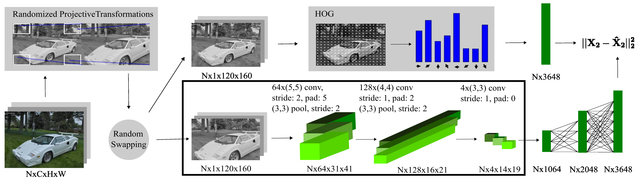
\includegraphics[width=\linewidth]{Bilder/CALC_Pipeline.jpg}
%    \caption{Pipeline CALC Algorithmus für Training}
%    \label{fig:CALC_1}
%\end{figure}
%
%%CALC ist Ein Algorithmus der auf Grundlage eines CNN's Loopclosures aus 2D Bilddaten Erkennen Soll. Das ziel der Entwickler war es dabei eine hohe Robustheit gegenüber Helligkeitsschwankungen und blickwinkeländerungen zu erreichen. Um das zu erreichen wurde ein CNN entsprechend trainiert. Der Vorteil des Verfahrens ist, dass das Training des Netzes unsupervised abläuft und daher kein aufwendig gelabelter Bilddatensatz benötigt wird.
%%Für die Merkmalsextraktion wird das HOG (Histogram of Oriented Gradients) verfahren genutzt. Das Verfahern wurde durch (ZITAT) das erste mal Vorgestellt. Merkmale für eine Klassifizierung werden dabei durch die Interpretation von stärke und Richtung von kanten in einem bestimmten Bildausschnitt erzeugt. Ein Bild wird dabei Raster artig abgetastet, die Ergebnisse werden in einem Histogramm je ihrer Ausrichtung nach Angeordnet.
%%
%
%
%CALC ist ein Algorithmus zur erkennung von Loop Closures in zweidimensionalen Bilddaten. Zur verwendung kommt dabei ein Konvolutional Neuronal Network, dass mit Augenmerk auf eine hohe Robustheit gegenüber Blickwinkel und Helligkeit  Veränderungen entwickelt und trainiert wurde. zudem ist das system für niedrige Hardwareanforderungen ausgelegt und benötigt im Gegensatz zu vergleichbaren Ansätzen wenig Rechnerressourcen. Gerade der geringen Ressourcen Anspruch macht es Prätendiert um es Parallel zu einem anderen Verfahren zu nutzen um dessen Genauigkeit zu erhöhen.\\
%Die Architektur das Trainings verdeutlicht wie die Angedachten ziele erreicht werden konnten. \\
%Als input für das Training können Bilddaten ohne labels verwendet werden, was die Auswahl geeigneter Trainingsdatensätze deutlich vereinfacht. Für das Training wird ein satz Bilder $\mathcal{I}$ mit N Bildern eingelesen. Schritt eins wandelt Farb- zunächst in Grauwertbiler um, dies fördert die Robustheit gegenüber Blickwinkeländerungen, da Farben je nach Lichteinfallswinkel unterschiedlich erkannt werden können. Die Bilder werden anschließend auf eine Größe von$ H x W = 120 x 160$ Pixeln reduziert. Da die Blickwinkelunabhängigkeit trainiert werden soll ohne das im Datensatz aufnahmen vorliegen, die orte in verschiedenen Perspektiven zeigen muss eine Blickwinkeländerung vor dem Training künstlich erzeugt werden. Bei jedem Bild $I$  aus dem Datensatz $\mathcal{I}$ wird in den Ecken ein Quadrat mit den Seitenlängen $H/4 x W/4$ definiert. Nun wird in jedem Rechteck ein Zufälliger Punkt gewählt. Anschließend wird eine Geometrische Transformation mit der Transformationsmatrix $H_p$ volzogen. Die zuvor gewählten Punkte entsprechen nach der Transformation den außen ecken des neu generierten Bildes $I_\omega$, diese Transformation ist in Abbildung \ref{fig:CALC_2} an einem Beispielbild zu sehen. Von jedem Bild aus dem Datensatz  $\mathcal{I}$liegen nun zwei Ansichten $I und I_\omega $ vor, daraus wird zufällig eine ausgewählt und einem HOG Deskriptor zugefügt. 
%
%
%Der von Navneet Dalal und Bill Triggs vorgestellte Algorithmus \textit{Historamm of oriented Gradients} \cite{Dalal2005} wurde als Objekterkennungsalgorithmus entwickelt um Fußgänger zu erkennen. Im allgemeinen ist es ein Verfahren um Feature Deskriptoren, bei HOG die sogenannten HOG diskriptoren zu erzeugen. In einem ersten schritt wird zunächst eine Farb- und Gammakompression durchgeführt. In unserem Fall stehen nur Grauwertbilder als Eingang zu Verfügung. Die Gammakompression nach Dalal und Triggs normiert dabei alle Bildpunkte mit der Quadratwurzelfunktion und dient dazu Robustheit gegenüber Helligkeitsänderungen zu erlangen. Als nächstes werden Pixelweise in x- und y- Richtung die Gradienten Errechnet. In Abbildung ..HOG.. sieht man die Gradientenbilder in x-Richtung (b), y-Richtung (c) und das dazugehörigen Original (a). Im Anschluss werden pro Pixel die Gradienten Magnitude $m$ sowie die Gradientenrichtung $\theta$ bestimmt.
%
% \begin{align}
%   m(x,y)=\vert\triangledown f(x,y)\vert=\sqrt{f_x^2+f_y^2}\\
%   \theta=arctan \frac{f_x}{f_y}  
%\end{align}
%
%Jeder Pixel besitzt nun einen Vektor mit bestimmter Länge und Richtung  wie in Abbildung Hog2 zu sehen. Im Folgenden schritt wird das Bild in Zellen unterteilt, wobei eine Zelle Beispielweise die größe von $8x8$ pixel besitzen kann. Von jedem Pixel wird die Magnitude in ein Histogramm eingetragen, die Richtungen sind dabei die sogenannten Bins. Es gibt 9 Bins für $0-180^\circ$, also $0,20,40,...,160$, wie in abbildung HOG3 zu sehen ist. Damit werden pro zelle die$8x8=64$ Pixel werte in einem 9 Felder großen Vektor gespeichert. Über diese Zellen wird ein Fenster geschoben, zum Beispiel mit der Größe $16 x 16$ Pixeln. Alle 9 stelligen Histogramm Vektoren, also in diesem Fall 4, werden nun Normalisiert um sie nocheinmal unabhängig gegenüber Helligkeitsveränderungen zu machen. Dafür werden  alle Histogramm Vektoren eines Blocks zum Vektor $v$ zusammengefasst. $\|v\|_k$ ist die k-Norm für k=1,2 und $e$ eine kleine Normierungskonstante. Dalal und Triggs erwähnen 3 Formeln die zur Normierung angewendet werden können und ähnliche Ergebnisse liefern,
%
%\begin{align}
%   L1-Norm  f=\frac{v}{\|v\|_1 +e}\\
%   L2-Norm  f=\frac{v}{\sqrt{\|v\|_k2^2 +e^2}}\\
%   L1_Wurzel-Norm  f=\sqrt{\frac{v}{\|v\|_1+e}}
%\end{align}
%
%Die Normalisierten vektoren der lokalen Blöcke werden im letzten Schritt  zu einem Merkmalsvektor, den schon erwähnten HOG Deskriptor, zusammengeführt stellen dann die HOG-Features dar. Die Deimension dieses Vektors ergibt sich dabei aus  $m x m$ zellen pro Block, $n_b$ Blöcken im Bild und $N$ Bins pro Histogramm. . In unserem Fall besitzt dieser Vektor die dimension $1x3648$. 
%
%So können die, Information die ein $ 160 x 120 = 19200 $ pixel Bild enthalten in einen Vektor der Größe $ 1 x 3648$ komprimiert werden. 
%Sind alle Bilder durch ein HOG Vektor beschrieben werden diese zusammengefügt und als $Nx3648$, wobei $N$ die Anzahl der Bilder im Trainingsdatensatz $\mathcal{I}$ darstellt, Vektor $X_2$ abgespeichert.\\
%Die nicht durch den HOG Algorithmus verarbeiteten Bildpaare werden in einem Vektor $X_1$ gespeichert. 
%Nun beginnt das eigentliche Training des CNN autoencoders. Das Netz versucht dabei $X_2$ durch die Eingabe von $X1$ zu Rekonstruieren.\\
%
%In Abbildung \ref{fig:CALC_1} is die Traniningspipeline zu sehen, das dafür entworfene Netz besitzt zwei hintereinander geschalteten Faltungsschichten welche jeweils ein angehängtes Pooling Layer besitzen. Darauf folgt noch eine einfache Faltungsschicht. Die Ausgabe dieser Faltungsschicht ist ein $1x1064$ Vektor.  Für das Training werden noch 3 fully connected layer angehängt um den HOG Diskriptor $Z2$ der form $1x3648$ zu Rekonstruieren. Dafür werden Sigmoid Aktivierungsfunktionen genutzt, da diese für eine Normierung sorgen (1,0). Für die Faltungsschichten hingegenen werden wie dafür allgemin gebräuchlich ReLU Aktivierungsfunktionen Verwendet. Um den das Rekonstruierte $\widehat{X_2}$ mit dem gesuchten $X_2$ zu vergleichen kommt eine $l_2 loss$ Funktion zum Einsatz.\\
%Wie schon erwähnt wird für den Livebetrieb die Rekonstruktion des HOG-Deskriptors nichtmehr benötigt, damit sinkt die Anzahl an schichten auf drei und macht das verfahren sehr ressourceneffizient. Die Extrahierten Diskriptoren werden im Livebetrieb in einer Datenbank gesichrt. Die suche nach passenden loop-closures erfolgt dann mithilfe einer einfachen Linearen Suche. Getestet wurde auch eine K-d Baumsuche, welche jedoch keinerlei Geschwindigkeitsvorteile brachte. \\
% Zusammengefasst lässt sich sagen das dieser Ansatz durch das Training, auf die beschrieben HOG-Diskiptoren, eine hohe Komprimierung auf der einen Seite und eine hohe Robustheit gegen Helligkeits- unterschiede auf der anderen Seite erzeugt. Die Künstlich generierte Blickwinkelverzerrung erzeugt eine gewisse Blinkwinkelrobustheit, nachteilig daran ist das die blinkwinkel nur bis zu einem gewissen maße verzerrt werden können, was jedoch wett gemacht werden kann da viel Größere Datensätze Verwendet werden können.\\
% Ein großer Anteil der Veröffentlichung von Merrill und Huang behandelt diverse Testszenarien in denen der Ansatz erfolgreich gegen verfahren wie \textit{Utoencoder, ALEXNet,LA, DBoW2, HOG}. CALC konnte sich selbst bei datensaätzen welche für das training der anderen Verfahren verwendet wurde durchsetzen und das mit geringeren Ressourcenanforderungen.
%
%
%
%
%
%. Darauf 
%
%Dafür werden lediglich zwei kombinierte Faltngs- und  pooling schichten verwendet. Ein reine Faltungsschicht und drei voll vernetzte Schichten. Jede Faltungsschicht hat eine ReLu (rectified layer) Aktvierung nach sich, wohingegen jede Voll verbundene Schicht  eine Sigmoindaktivierung besitzt. 
%
%
%
%
%
%The training network aims to reconstruct X2 given X1
%using only two convolution and pooling paired layers, one
%pure convolution layer, and three fully-connected layers. Note
%that every layer has an activation after it. We use the rectified
%linear unit (ReLU) activation for the convolutional layers,
%while the sigmoid activation is chosen for the fully connected
%layers in order to better reconstruct the HOG descriptor (as
%it normalizes the data into [0,1]). Additionally, since the
%Euclidean distance is naturally a good
%%
%%
%%Die Merkmale bestehen dabei aus Blöcken von Histogrammen von Gerichteten Gradienten. 
%%
%%
%%
%%
%% zur Objekterkennung , ist und Bilderkennung Ziel ist es dabei aus zweidimensionalen Bildern, hier von mit der größe 120x160, wichtige Merkmale zu extrahieren und sie in einem  Vektor der größe 1x3648 zu speichern.
%%
%% der form  Dabei ist enscheident nutzvolle von nutzlosen informationen in Bildern zu trennen um eine Datenreduktion zu erzeugen. Typischer Einsatzzweck von HOG Deskriptoren 
%%
%%
%%
%%
%%
%%
%%
%%
%%
%%
%%
%%
%%
%%
%%
%%
%%
%%
%%
%%
%%In diesem fall dient es dazu das Neuronale netz auf helligkeits, blickwinkel und Datenreduktion zu trainieren
%
%
%\begin{figure}
%    \centering
%    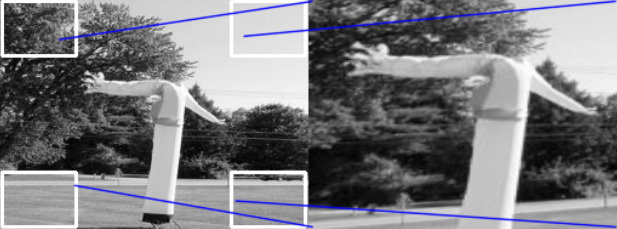
\includegraphics[width=\linewidth]{Bilder/CALC_beispiel_trainingstransformation.jpg}
%    \caption{Beispiel für ein Trainingsbildpaar. Links vor rechts nach der Geometrischen Transformation. Es entsteht dabei sowohl eine Bildverzerrung als auch eine Zoom Effekt.}
%    \label{fig:CALC_2}
%\end{figure}
%
%%
%%Großer VOrteil des systems ist die Gute Trainierbarkeit von 
%%
%%
%%Input der Trainingsdaten sind einfache ungelabelte bilder, da das Training unsuperwised 
%%
%%
%
%
%%Ein Histogram of Oriented Gradients (HOG) bezeichnet die Anordnung der Gradienten eines Samples innerhalb eines Histogramms. Die Arbeit von [Dal06] stellte das Verfahren erstmals im Rahmen der Doktorarbeit vor und erzielte bis dahin sehr gute Ergebnisse. Als Merkmal für eine Objektklassifizierung werden die Gradienten interpretiert, d.h. die Richtung und Stärke von Kanten in einem festgelegten Bildausschnitt. Die Gradienten werden für Teilausschnitte des Samples in einem Histogramm nach ihrer Ausrichtung angeordnet. Die Betrachtung des entstehenden Vektors reduziert zum einen die Dimensionalität des 2D-Bildes auf einen 1D- Vektor und begünstigt so schnellere Rechenzeiten der Klassifikation. Zum anderen werden durch die Anordnung der Merkmale in einem Histogramm die Farb- und Intensitätswerte des Bildes quasi geglättet, was durch eine Normalisierung der Gradienten gestärkt wird.
%
%%
%%
%%Wie auch der Segmap Algorithmus basiert auch CALC auf einem CNN.  CALC ist ein Verfahren, das Ausschließlich für die Verwendung von Zwei Kameras konziert ist. Die Schwierigkeit die Bei der Verwendung von 2 dimensionalen FBIldern  auftritt ist die, das blickwinkel und helligkeit maßgeblichen einfluss auf die wiedererkennbarkeit von zuvor gesehenen umgebungen haben. Der Ansatz wurde spiziell so entwickelt das er diese schwierigen gegebnheiten meistern kann. In abbildung ... wird der Stukturelle Aufbau des Verfahrens gezeigt. \\
%%Kernelemnt des Verfahrens stellt das ... Layerige CNN dar. Zum trainieren sind keine glabelte daten von nöten welhalb die Idee unter Unsupervised learning zu Betrachten ist. Hierbei können ungelabelte Daten zum Training des Algorithmus herangezogen werden, was die suche nach geeigneten Trainingstaten Maßiv vereinfacbhht. Zum Training wird zunächst ein bild vorverarbeitet.\\
%%Im Ersten Schritt werden vier boxen an den Ecken des bildet gelegt. dann werden zu  innerhalb dieser boxen durch zufallszahlen punkte bestimmt. Siehe Abbildung ... Nun werden verschiedene versionen mit unterschiedlichen verzerrungen und Zoomstufen erstellt Zudem werden Farbbilder in Schwarzweißbilder gewandelt um.  Als Input dienen Bildersequenzen und eine Odometryinformation. In einem Hersten
%%
%
%\section{Fusionierung}
%mit Vision Ansatz (muss nicht neu trainiert werden)
%
%Gewichtet
%
%Erkennung wenn RGB zu dunkel, dann nur Segmap zb wenn durchschnitt aller Pixelwerte unter bestimmter grenze liegen 
